%!TEX TS-program = xelatex
\documentclass[11pt]{article}

\usepackage[english]{babel}

\usepackage{amsmath,amssymb,amsfonts}
\usepackage[utf8]{inputenc}
\usepackage[T1]{fontenc}
\usepackage{stix2}
\usepackage[scaled]{helvet}
\usepackage[scaled]{inconsolata}

\usepackage{lastpage}

\usepackage{setspace}

\usepackage{ccicons}

\usepackage[hang,flushmargin]{footmisc}

\usepackage{geometry}

\setlength{\parindent}{0pt}
\setlength{\parskip}{6pt plus 2pt minus 1pt}

\usepackage{fancyhdr}
\renewcommand{\headrulewidth}{0pt}\providecommand{\tightlist}{%
  \setlength{\itemsep}{0pt}\setlength{\parskip}{0pt}}

\makeatletter
\newcounter{tableno}
\newenvironment{tablenos:no-prefix-table-caption}{
  \caption@ifcompatibility{}{
    \let\oldthetable\thetable
    \let\oldtheHtable\theHtable
    \renewcommand{\thetable}{tableno:\thetableno}
    \renewcommand{\theHtable}{tableno:\thetableno}
    \stepcounter{tableno}
    \captionsetup{labelformat=empty}
  }
}{
  \caption@ifcompatibility{}{
    \captionsetup{labelformat=default}
    \let\thetable\oldthetable
    \let\theHtable\oldtheHtable
    \addtocounter{table}{-1}
  }
}
\makeatother

\usepackage{array}
\newcommand{\PreserveBackslash}[1]{\let\temp=\\#1\let\\=\temp}
\let\PBS=\PreserveBackslash

\usepackage[breaklinks=true]{hyperref}
\hypersetup{colorlinks,%
citecolor=blue,%
filecolor=blue,%
linkcolor=blue,%
urlcolor=blue}
\usepackage{url}

\usepackage{caption}
\setcounter{secnumdepth}{0}
\usepackage{cleveref}

\usepackage{graphicx}
\makeatletter
\def\maxwidth{\ifdim\Gin@nat@width>\linewidth\linewidth
\else\Gin@nat@width\fi}
\makeatother
\let\Oldincludegraphics\includegraphics
\renewcommand{\includegraphics}[1]{\Oldincludegraphics[width=\maxwidth]{#1}}

\usepackage{longtable}
\usepackage{booktabs}

\usepackage{color}
\usepackage{fancyvrb}
\newcommand{\VerbBar}{|}
\newcommand{\VERB}{\Verb[commandchars=\\\{\}]}
\DefineVerbatimEnvironment{Highlighting}{Verbatim}{commandchars=\\\{\}}
% Add ',fontsize=\small' for more characters per line
\usepackage{framed}
\definecolor{shadecolor}{RGB}{248,248,248}
\newenvironment{Shaded}{\begin{snugshade}}{\end{snugshade}}
\newcommand{\KeywordTok}[1]{\textcolor[rgb]{0.13,0.29,0.53}{\textbf{#1}}}
\newcommand{\DataTypeTok}[1]{\textcolor[rgb]{0.13,0.29,0.53}{#1}}
\newcommand{\DecValTok}[1]{\textcolor[rgb]{0.00,0.00,0.81}{#1}}
\newcommand{\BaseNTok}[1]{\textcolor[rgb]{0.00,0.00,0.81}{#1}}
\newcommand{\FloatTok}[1]{\textcolor[rgb]{0.00,0.00,0.81}{#1}}
\newcommand{\ConstantTok}[1]{\textcolor[rgb]{0.00,0.00,0.00}{#1}}
\newcommand{\CharTok}[1]{\textcolor[rgb]{0.31,0.60,0.02}{#1}}
\newcommand{\SpecialCharTok}[1]{\textcolor[rgb]{0.00,0.00,0.00}{#1}}
\newcommand{\StringTok}[1]{\textcolor[rgb]{0.31,0.60,0.02}{#1}}
\newcommand{\VerbatimStringTok}[1]{\textcolor[rgb]{0.31,0.60,0.02}{#1}}
\newcommand{\SpecialStringTok}[1]{\textcolor[rgb]{0.31,0.60,0.02}{#1}}
\newcommand{\ImportTok}[1]{#1}
\newcommand{\CommentTok}[1]{\textcolor[rgb]{0.56,0.35,0.01}{\textit{#1}}}
\newcommand{\DocumentationTok}[1]{\textcolor[rgb]{0.56,0.35,0.01}{\textbf{\textit{#1}}}}
\newcommand{\AnnotationTok}[1]{\textcolor[rgb]{0.56,0.35,0.01}{\textbf{\textit{#1}}}}
\newcommand{\CommentVarTok}[1]{\textcolor[rgb]{0.56,0.35,0.01}{\textbf{\textit{#1}}}}
\newcommand{\OtherTok}[1]{\textcolor[rgb]{0.56,0.35,0.01}{#1}}
\newcommand{\FunctionTok}[1]{\textcolor[rgb]{0.00,0.00,0.00}{#1}}
\newcommand{\VariableTok}[1]{\textcolor[rgb]{0.00,0.00,0.00}{#1}}
\newcommand{\ControlFlowTok}[1]{\textcolor[rgb]{0.13,0.29,0.53}{\textbf{#1}}}
\newcommand{\OperatorTok}[1]{\textcolor[rgb]{0.81,0.36,0.00}{\textbf{#1}}}
\newcommand{\BuiltInTok}[1]{#1}
\newcommand{\ExtensionTok}[1]{#1}
\newcommand{\PreprocessorTok}[1]{\textcolor[rgb]{0.56,0.35,0.01}{\textit{#1}}}
\newcommand{\AttributeTok}[1]{\textcolor[rgb]{0.77,0.63,0.00}{#1}}
\newcommand{\RegionMarkerTok}[1]{#1}
\newcommand{\InformationTok}[1]{\textcolor[rgb]{0.56,0.35,0.01}{\textbf{\textit{#1}}}}
\newcommand{\WarningTok}[1]{\textcolor[rgb]{0.56,0.35,0.01}{\textbf{\textit{#1}}}}
\newcommand{\AlertTok}[1]{\textcolor[rgb]{0.94,0.16,0.16}{#1}}
\newcommand{\ErrorTok}[1]{\textcolor[rgb]{0.64,0.00,0.00}{\textbf{#1}}}
\newcommand{\NormalTok}[1]{#1}

\newlength{\cslhangindent}
\setlength{\cslhangindent}{1.5em}
\newlength{\csllabelwidth}
\setlength{\csllabelwidth}{3em}
\newenvironment{CSLReferences}[3] % #1 hanging-ident, #2 entry spacing
 {% don't indent paragraphs
  \setlength{\parindent}{0pt}
  % turn on hanging indent if param 1 is 1
  \ifodd #1 \everypar{\setlength{\hangindent}{\cslhangindent}}\ignorespaces\fi
  % set entry spacing
  \ifnum #2 > 0
  \setlength{\parskip}{#2\baselineskip}
  \fi
 }%
 {}
\usepackage{calc} % for \widthof, \maxof
\newcommand{\CSLBlock}[1]{#1\hfill\break}
\newcommand{\CSLLeftMargin}[1]{\parbox[t]{\maxof{\widthof{#1}}{\csllabelwidth}}{#1}}
\newcommand{\CSLRightInline}[1]{\parbox[t]{\linewidth}{#1}}
\newcommand{\CSLIndent}[1]{\hspace{\cslhangindent}#1}\geometry{verbose,letterpaper,tmargin=2.2cm,bmargin=2.2cm,lmargin=2.2cm,rmargin=2.2cm}

\usepackage{lineno}
% \usepackage[nolists,noheads]{endfloat}

\usepackage{floatrow}

\floatsetup[figure]{
              floatwidth=\textwidth}

\pagestyle{plain}

\tolerance=1
\emergencystretch=\maxdimen
\hyphenpenalty=10000
\hbadness=10000

\doublespacing

\fancypagestyle{normal}
{
  \fancyhf{}
  \fancyfoot[R]{\footnotesize\sffamily\thepage\ of \pageref*{LastPage}}
}
\begin{document}
\raggedright
\thispagestyle{empty}
{\Large\bfseries\sffamily The missing link: discerning true from false
negatives when sampling species interaction networks}
\vskip 5em

%
\href{https://orcid.org/0000-0002-6506-6487}{Michael D.\,Catchen}%
%
\,\textsuperscript{1,2}\quad %
\href{https://orcid.org/0000-0002-0735-5184}{Timothée\,Poisot}%
%
\,\textsuperscript{3,2}\quad %
\href{https://orcid.org/0000-0002-6004-4027}{Laura J.\,Pollock}%
%
\,\textsuperscript{1,2}\quad %
\href{https://orcid.org/0000-0001-6075-8081}{Andrew\,Gonzalez}%
%
\,\textsuperscript{1,4}

\textsuperscript{1}\,McGill University\quad \textsuperscript{2}\,Québec
Centre for Biodiversity Sciences\quad \textsuperscript{3}\,Université de
Montréal\quad \textsuperscript{4}\,Québec Centre for Biodiversity
Science


\textbf{Correspondance to:}\\
Michael D. Catchen --- \texttt{michael.catchen@mcgill.ca}\\

\vfill
This work is released by its authors under a CC-BY 4.0 license\hfill\ccby\\
Last revision: \emph{\today}

\clearpage
\thispagestyle{empty}

\vfill


        {\bfseries Abstract:}\,Ecosystems are composed of networks of
interacting species. These interactions allow communities of species to
persist through time through both neutral and adaptive processes.
Despite their importance, a robust understanding of (and ability to
predict and forecast) interactions among species remains elusive. This
knowledge-gap is largely driven by a shortfall of data---although
species occurrence data has rapidly increased in the last decade,
species interaction data has not kept pace, largely due to the intrinsic
difficulty and effort required to sample interactions. This means there
are many interactions between species that occur in nature, but we do
not think this interaction occurs because we have no record of it. These
so-called ``false-negatives'' bias data and hinder inference about the
structure and dynamics of interaction networks. Here, we demonstrate the
realized rate of false-negatives in data can be quite high, even in
thoroughly sampled systems, due to the intrinsic variation in abundances
across species in a community. We illustrate how a null model of
occurrence detection can be used to estimate the false-negative rate in
a given dataset. We also show how to directly incorporate uncertainty
due to observation error into model-based predictions of interaction
probabilities between species. One hypothesis is that interactions
between ``rare'' species are themselves rare because these species are
less likely to encounter one-another than species of higher relative
abundance, and that this can (in part) explain the common pattern of
nestedness in bipartite interaction networks. However, we demonstrate
that across several datasets of spatial or temporally replicated
networks, there are positive associations between species co-occurrence
and interactions, which suggests these interactions among ``rare''
species actually exist but simply are not observed. Finally, we assess
how false negatives influence various models of network prediction, and
recommend directly accounting for observation error in predictive
models. We conclude by discussing how the understanding of
false-negatives can inform how we design monitoring schemes for species
interactions.\\%
    
\vfill

\clearpage
\linenumbers
\pagestyle{normal}

\hypertarget{introduction}{%
\section{Introduction}\label{introduction}}

Species interactions drive many processes in evolution and ecology. A
better understanding of species interactions is an imperative to
understand the evolution of life on Earth, to mitigate the impacts of
anthropogenic change on biodiversity (Makiola \emph{et al.} 2020), and
for predicting zoonotic spillover of disease to prevent future pandemics
(Becker \emph{et al.} 2021). At the moment we lack sufficient data to
meet these challenges (Poisot \emph{et al.} 2021), largely because
species interactions are hard to sample (Jordano 2016). Over the past
few decades biodiversity data has become increasingly available through
remotely collected data and adoption of open data practices (Kenall
\emph{et al.} 2014; Stephenson 2020). Still, interaction data remains
relatively scarce because sampling typically requires human observation.
This induces a constraint on the amount, spatial scale, and temporal
frequency of resulting data that it is feasible to collect by humans.
Many crowdsourced methods for biodiversity data aggregation (e.g.~GBIF,
eBird) still rely on automated identification of species, which does not
easily generalize to interaction sampling. There is interest in using
remote methods for interaction sampling, which primarily detect
co-occurrence and derive properties like species avoidance from this
data (Niedballa \emph{et al.} 2019). However, co-occurrence itself is
not necessarily indicative of an interaction (Blanchet \emph{et al.}
2020). This is an example of semantic confusion around the word
``interaction''---for example one might consider competition a type of
species interaction, even though it is marked by a lack of co-occurrence
between species, unlike other types of interactions, like predation or
parasitism, which require both species to be together at the same place
and time. Here we consider interaction in the latter sense, where two
species have fitness consequences on one-another if (and only if) they
are in the sample place at the same time. In addition, here we only
consider direct (not higher-order) interactions.

We cannot feasibly observe all (or even most) of the interactions that
occur in an ecosystem. This means we can be confident two species
actually interact if we have a record of it (assuming they are correctly
identified), but not at all confident that a pair of species \emph{do
not} interact if we have \emph{no record} of those species observed
together. In other words, it is difficult to distinguish
\emph{true-negatives} (two species never interact) from
\emph{false-negatives} (two species interact sometimes, but we do not
have a record of this interaction). For a concrete example of a
false-negative in a food web, see fig.~\ref{fig:concept}. Because even
the most highly sampled systems will still contain false-negatives,
there is increasing interest in combining species-level data
(e.g.~traits, abundance, range, phylogenetic relatedness, etc.) to build
models to predict interactions between species we haven't observed
together before (Strydom \emph{et al.} 2021). However, the noise of
false-negatives could impact the efficacy of our predictive models and
have practical consequences for answering questions about interactions
(de Aguiar \emph{et al.} 2019). This data constraint is amplified as the
interaction data we have is geographically biased toward the usual
suspects (Poisot \emph{et al.} 2021). We therefore need a statistical
approach to assessing these biases in the observation process and their
consequences for our understanding of interaction networks.

The importance of \emph{sampling effort} and its impact on resulting
ecological data has produced a rich body of literature.The recorded
number of species in a dataset or sample depends on the total number of
observations (Walther \emph{et al.} 1995; Willott 2001), as do estimates
of population abundance (Griffiths 1998). This relationship between
sampling effort and spatial coverage and species detectability has
motivated more quantitatively robust approaches to account for error in
sampling data in many contexts: to determine if a given species is
extinct (Boakes \emph{et al.} 2015), to determine sampling design (Moore
\& McCarthy 2016), and to measure species richness across large scales
(Carlson \emph{et al.} 2020). In the context of interactions, an initial
concern was the compounding effects of limited sampling effort combined
with the amalgamation of data (across both study sites, time of year,
and taxonomic scales) could lead any empirical set of observations to
inadequately reflect the reality of how species interact (Paine 1988) or
the structure of the network as a whole (Martinez \emph{et al.} 1999;
McLeod \emph{et al.} 2021). Martinez \emph{et al.} (1999) showed that in
a plant-endophyte trophic network, network connectance is robust to
sampling effort, but this was done in the context of a system for which
observation of 62,000 total interactions derived from 164,000
plant-stems was feasible. In some systems (e.g.~megafauna food-webs)
this many observations is either impractical or infeasible due to the
absolute abundance of the species in question.

The intrinsic properties of ecological communities create several
challenges for sampling: first, species are not observed with equal
probability---we are much more likely to observe a species of high
abundance than one of very low abundance (Poisot \emph{et al.} 2015).
Canard \emph{et al.} (2012) presents a null model of food-web structure
where species encounter one-another in proportion to each species'
relative-abundance. This assumes that there are no associations in
species co-occurrence due to an interaction (perhaps because this
interaction is ``important'' for both species; Cazelles \emph{et al.}
(2016)), but in this paper we later show increasing strength of
associations leads to increasing probability of false-negatives in
interaction data, and that these positive associations are common in
existing network data. Second, observed co-occurrence is often equated
with meaningful interaction strength, but this is not necessarily the
case (Blanchet \emph{et al.} 2020)---a true ``non-interaction'' would
require that neither of two species, regardless of whether they
co-occur, ever exhibit any meaningful effect on the fitness of the
other. So, although co-occurrence is not directly indicative of an
interaction, it \emph{is} a precondition for an interaction.

Here, we illustrate how our confidence that a pair of species never
interacts highly depends on sampling effort. We demonstrate how the
realized false-negative-rate of interactions is related to the relative
abundance of the species pool, and introduce a method to produce a null
estimate of the false-negative-rate given total sampling effort (the
total count of all interactions seen among all species-pairs) and a
method for including uncertainty into model predictions of interaction
probabilities to account for observation error. We then confront these
models with data, by showing that positive associations in co-occurrence
data can increase the realized number of false-negatives and by showing
these positive associations are rampant in network datasets. We conclude
by recommending that the simulation of sampling effort and species
occurrence can and should be used to help design surveys of species
interaction diversity (Moore \& McCarthy 2016), and by advocating use of
null models like those presented here as a tool for both guiding design
of surveys of species interactions and for including detection error
into predictive models.

\begin{figure}
\hypertarget{fig:concept}{%
\centering
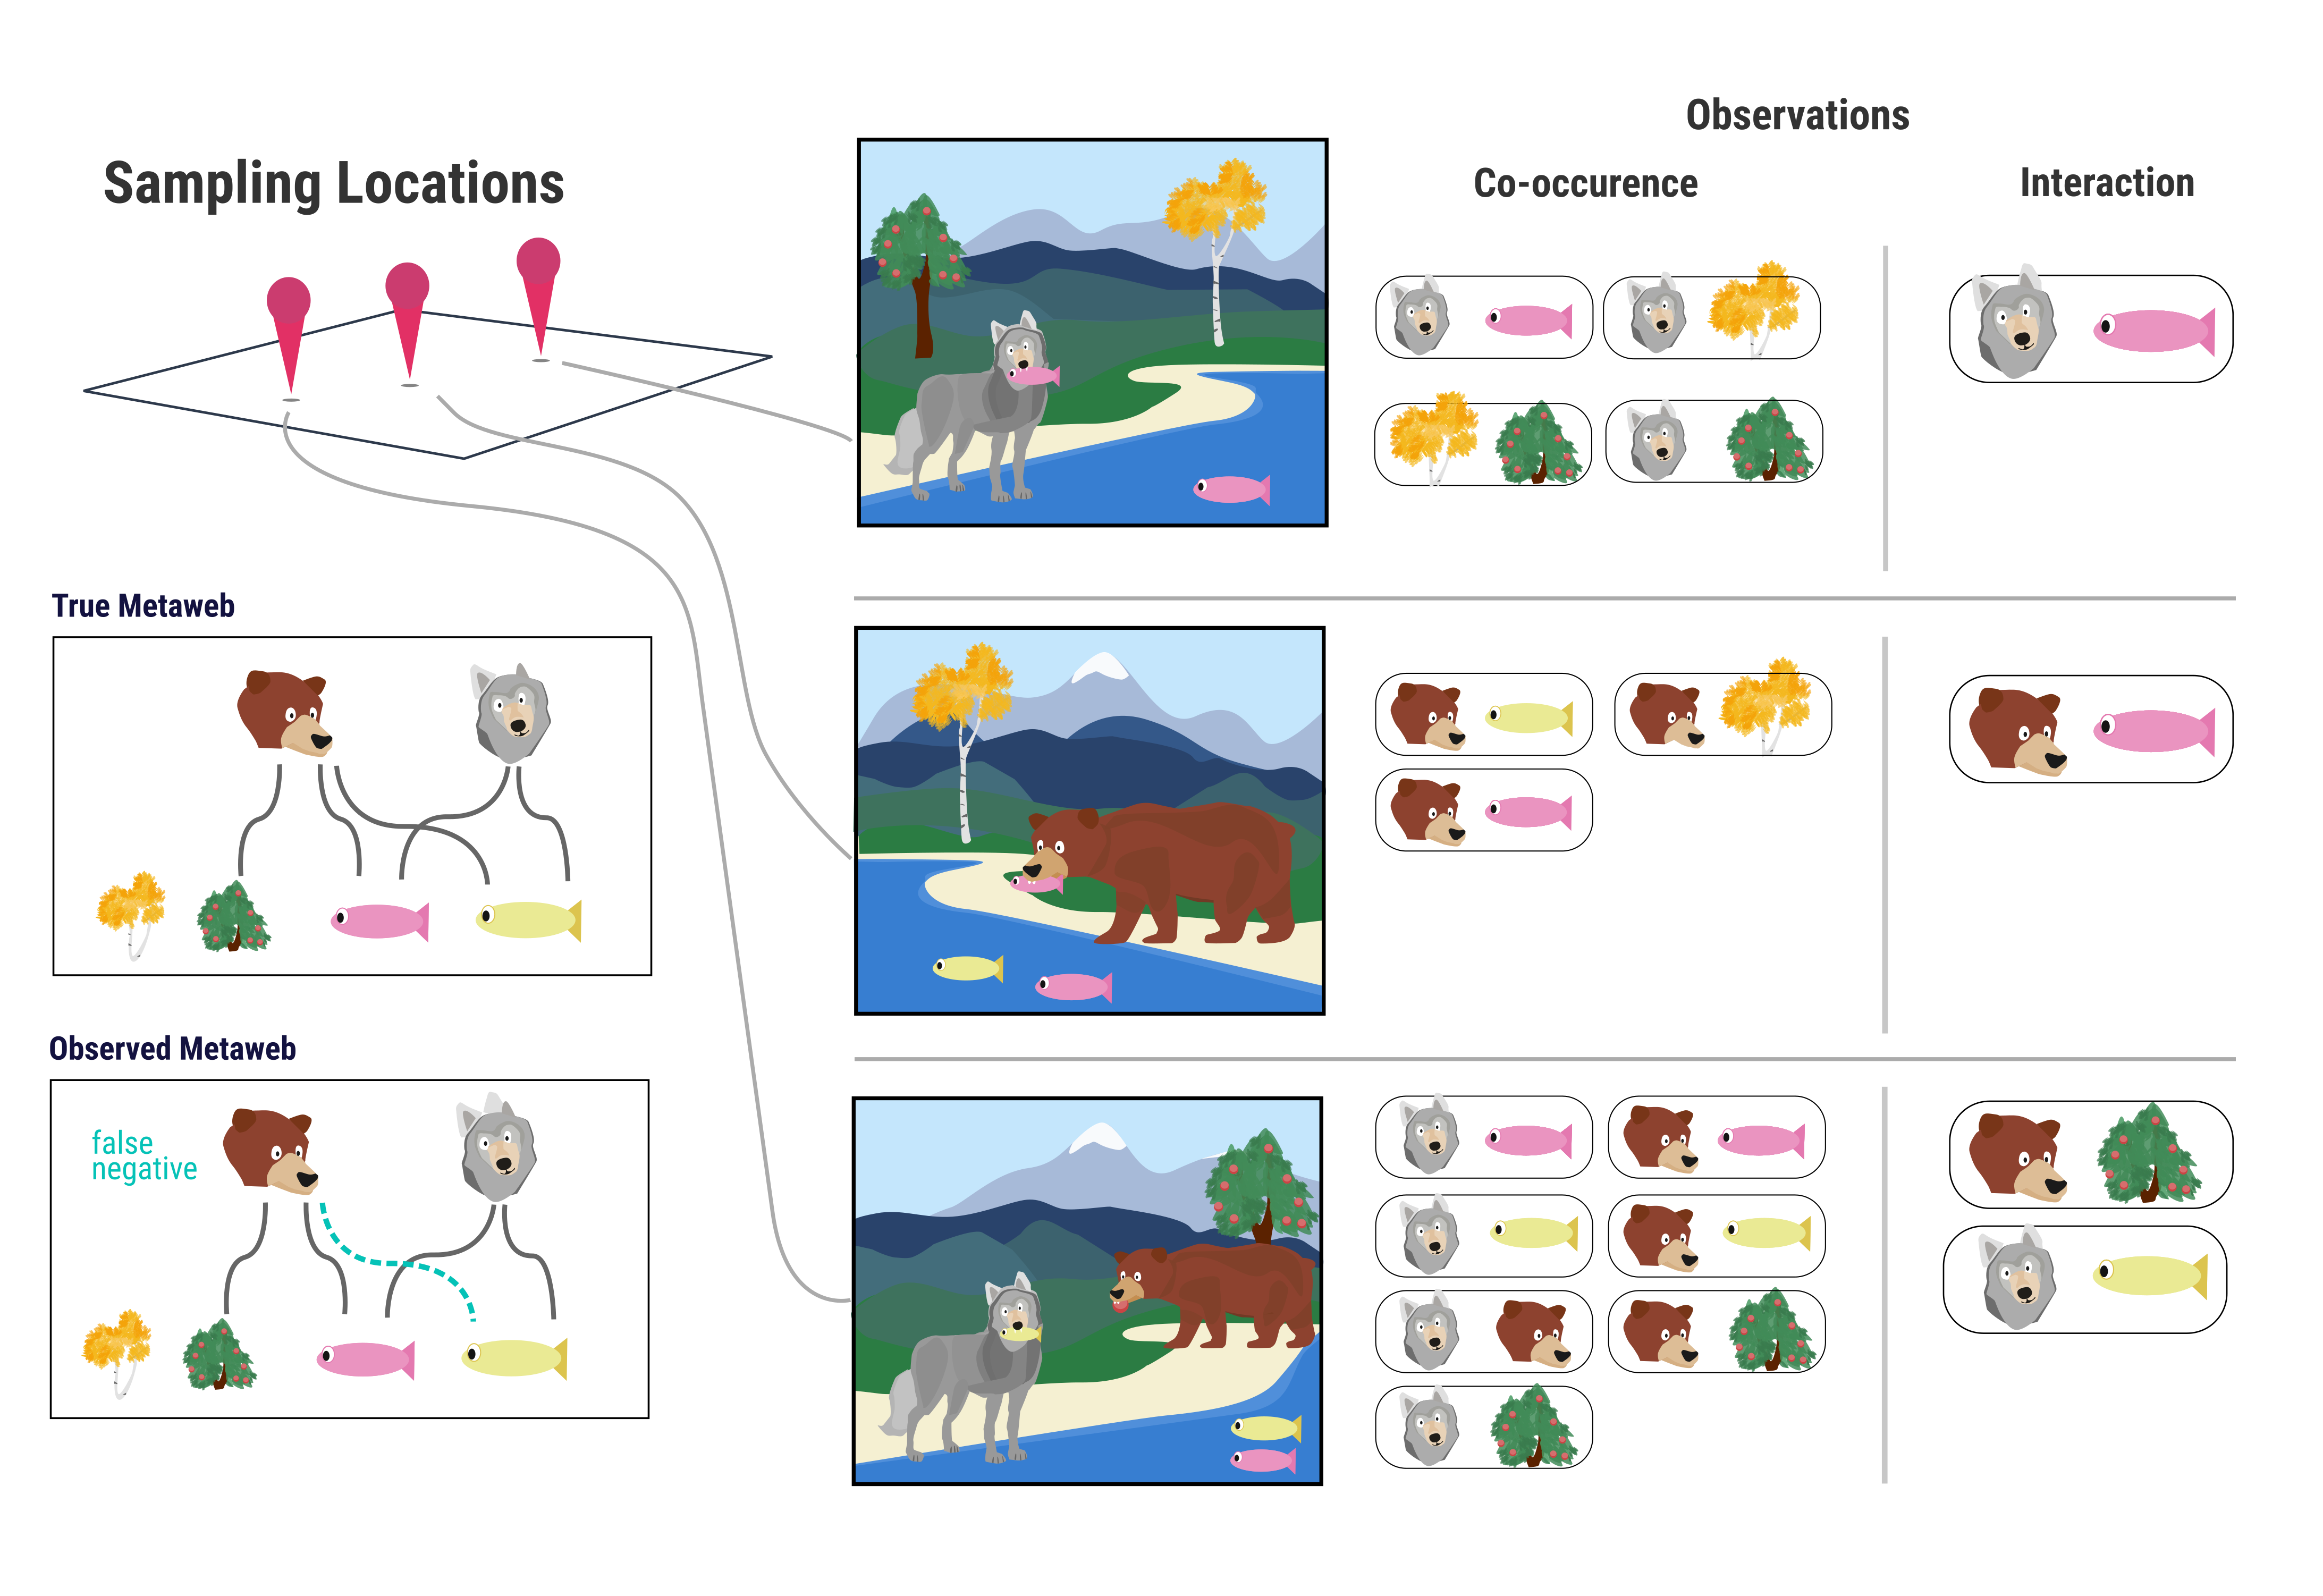
\includegraphics{./figures/concept.png}
\caption{This conceptual example considers a sample of the trophic
community of bears, wolves, salmon (pink fish), pike (yellow fish),
berry trees, and aspen trees. The true metaweb (all realized
interactions across the entire spatial extent) is shown on the left. In
the center is what a hypothetical ecologist samples at each site. Notice
that although bears are observed co-occurring with both salmon and pike,
there was never a direct observation of bears eating pike, even though
they actually do. Therefore, this interaction between bears and pike is
a false-negative.}\label{fig:concept}
}
\end{figure}

\hypertarget{accounting-for-false-negatives-in-species-interactions}{%
\section{Accounting for false-negatives in species
interactions}\label{accounting-for-false-negatives-in-species-interactions}}

In this section, we demonstate how difference in relative-abundance can
lead to many false-negatives in interaction data. We also introduce a
method for producing a null estimate of the false-negative-rate in
datasets via simulation, and a method for incorporating uncertainty
directly into predictions of species interactions to account for
observation error.

\hypertarget{how-many-observations-of-a-non-interaction-do-we-need-to-be-confident-its-a-true-negative}{%
\subsection{How many observations of a non-interaction do we need to be
confident it's a true
negative?}\label{how-many-observations-of-a-non-interaction-do-we-need-to-be-confident-its-a-true-negative}}

We start with a naive model of interaction detection: we assume that
every interacting pair of species is incorrectly observed as
not-interacting with an independent and fixed probability, which we
denote \(p_{fn}\) and subsequently refer to as the False-Negative-Rate
(FNR). If we observe the same species not-interacting \(N\) times, then
the probability of a true-negative (denoted \(p_{tn}\)) is given by
\(p_{tn}=1-(p_{fn})^N\). This relation (the probability-mass-function of
geometric distribution, a special case of the negative-binomial
distribution) is shown in fig.~\ref{fig:geometric}(A) for varying values
of \(p_{fn}\) and illustrates a fundamental link between our ability to
reliably say an interaction doesn't exist---\(p_{tn}\)---and the number
of times \(N\) we have observed a given species. In addition, note that
there is no non-zero \(p_{fn}\) for which we can ever \emph{prove} that
an interaction does not exist---no matter how many observations of
non-interactions \(N\) we have, \(p_{tn}<1\).

From fig.~\ref{fig:geometric}(A) it is clear that the more often we see
two species co-occurring, but \emph{not interacting}, the more likely
the interaction is a true-negative. This has several practical
consequences: first it means negatives taken outside the overlap of the
range of each species aren't informative because co-occurrence was not
possible, and therefore neither was an interaction. Second, we can use
this relation to compute the expected number of total observations
needed to obtain a ``goal'' number of observations of a particular pair
of species (fig.~\ref{fig:geometric}(B)). As an example, if we
hypothesize that \(A\) and \(B\) do not interact, and we want to see
species \(A\) and \(B\) both co-occurring and \emph{not interacting} 10
times to be confident this is a true negative, then we need an expected
1000 observations of all species if the relative abundances of \(A\) and
\(B\) are both \(0.1\).

Because the true FNR is latent, we can never actually be sure what the
actual number of false-negatives in our data---however, we can use
simulation to estimate the FNR for datasets of a given size using
neutral models of observation. If some of the ``worst-case'' FNRs
presented in fig.~\ref{fig:geometric}(A) seem unrealistically high,
considering that species are observed in proportion to their relative
abundance. In the next section we demonstrate that the distribution of
abundance in ecosystems can lead to very high realized values of FNR
(\(p_{fn}\)) simply as an artifact of sampling effort.

\begin{figure}
\hypertarget{fig:geometric}{%
\centering
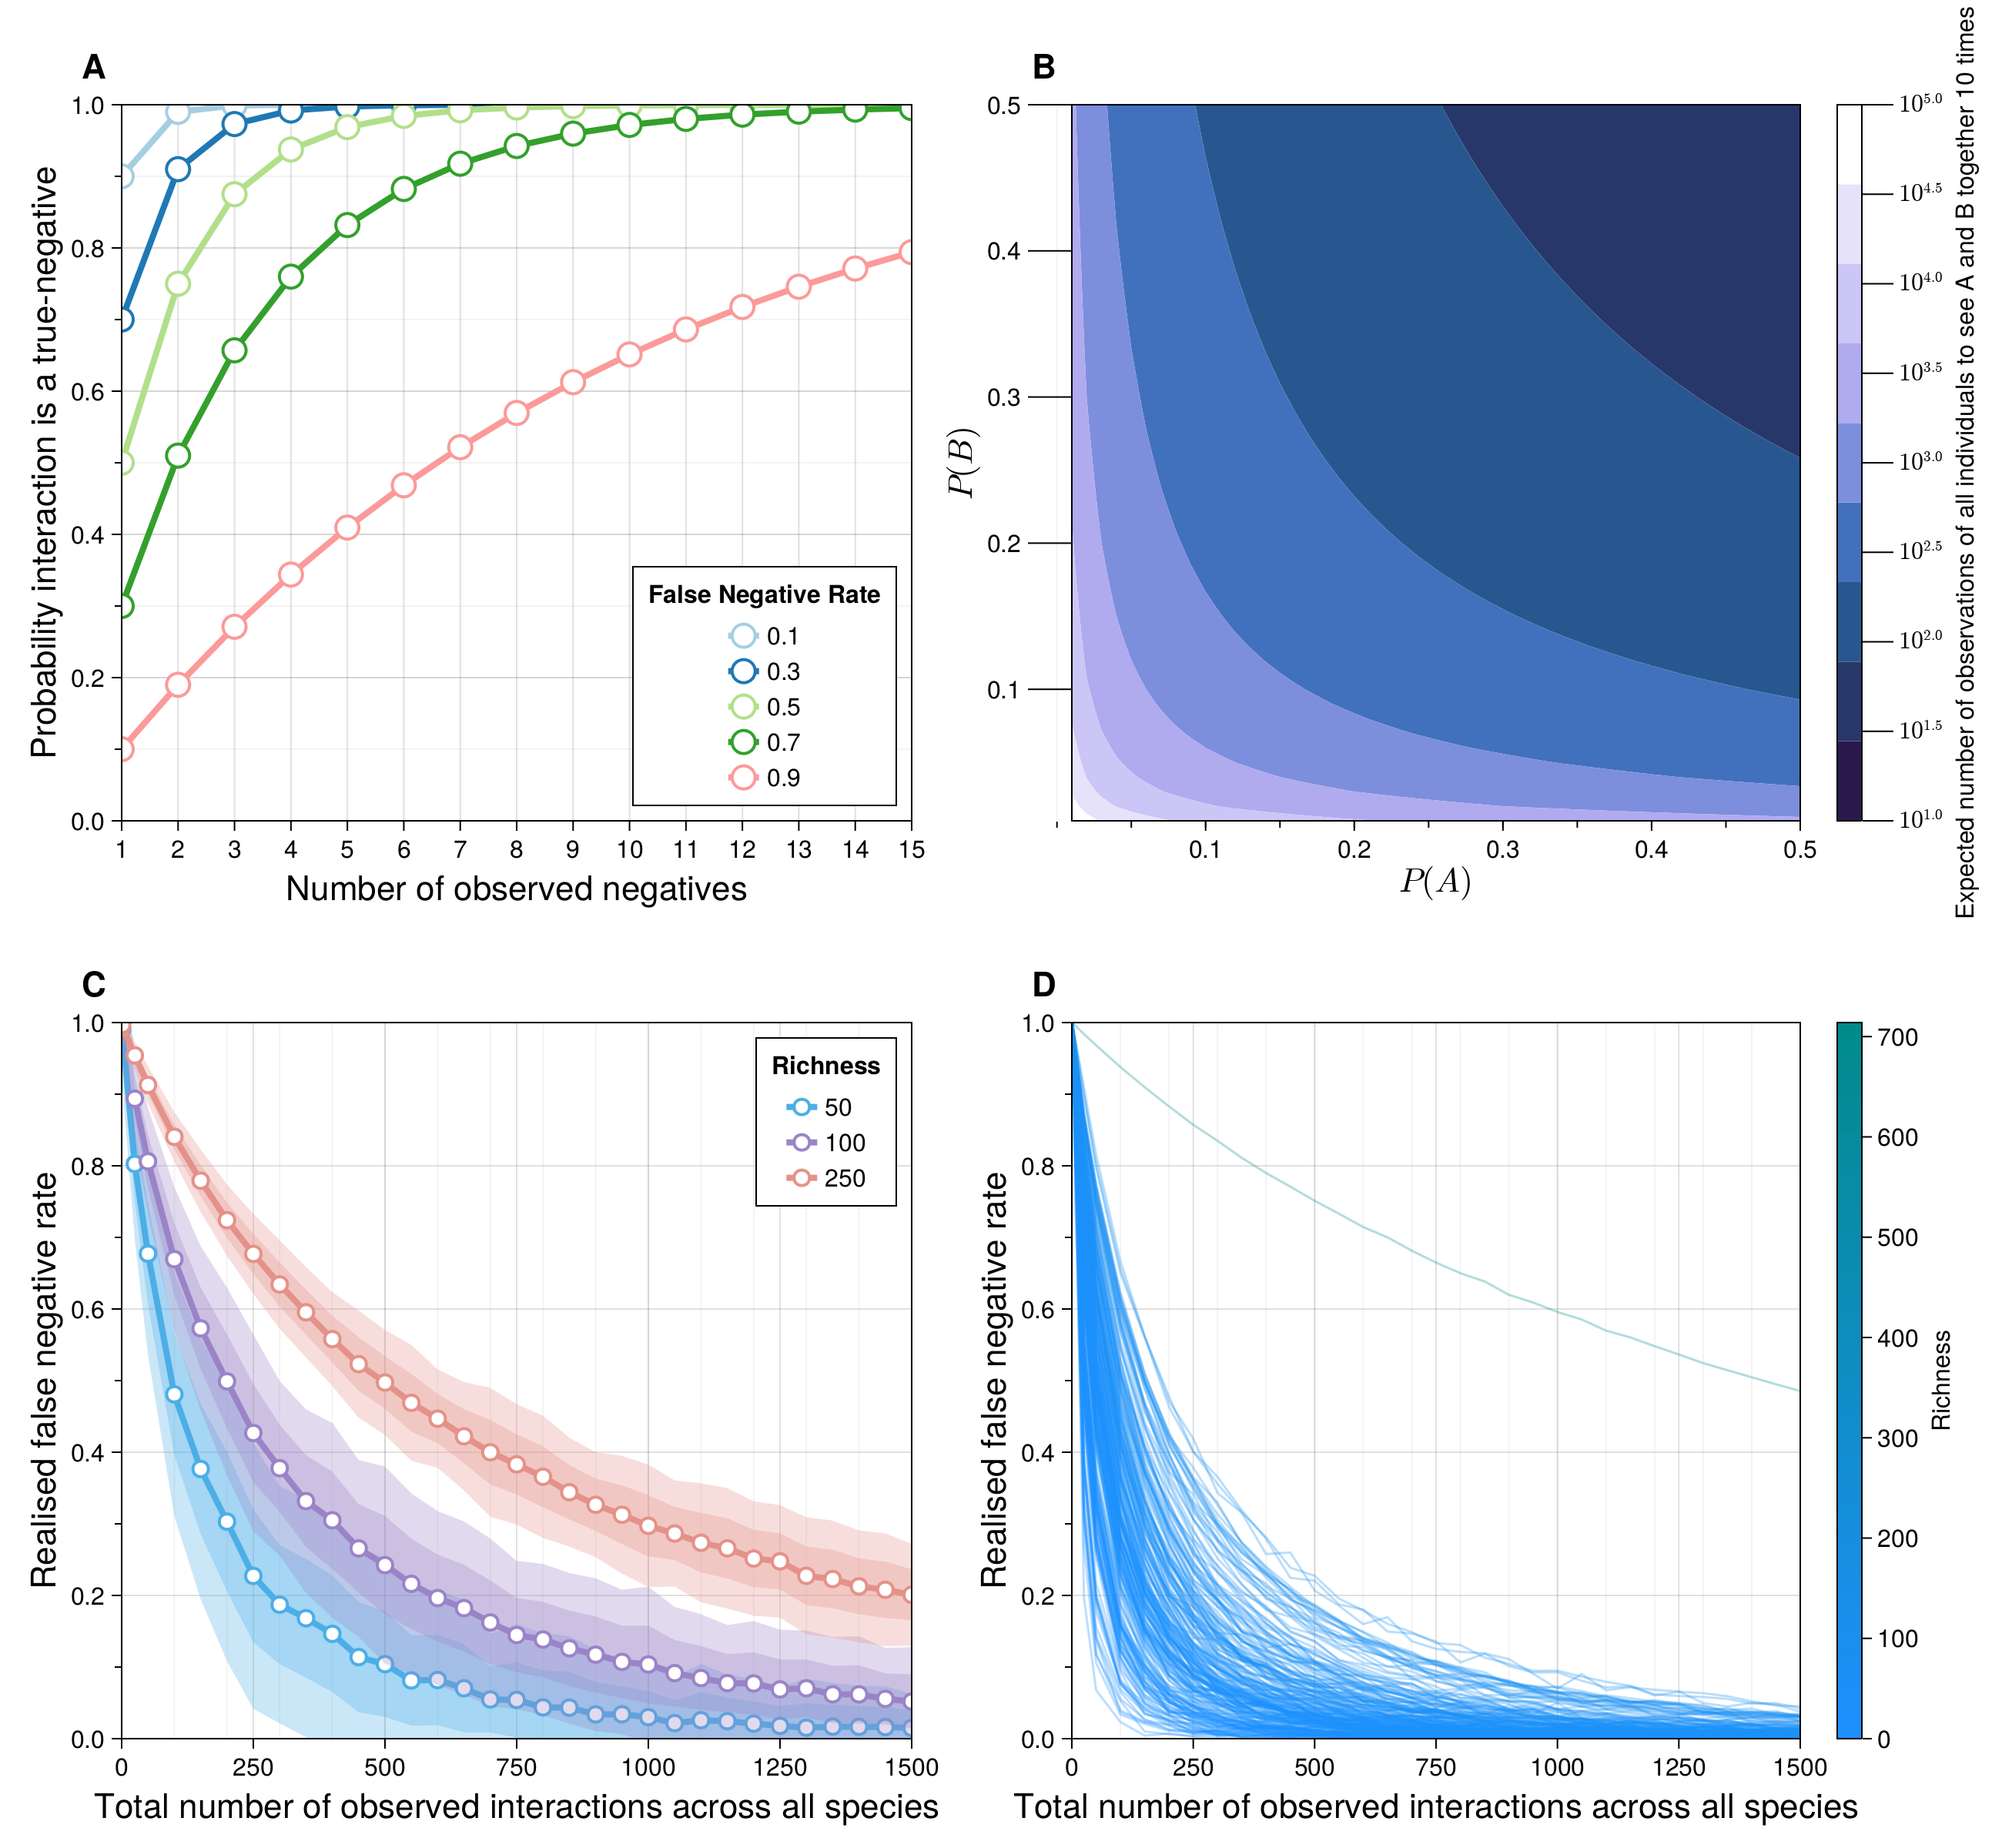
\includegraphics{./figures/fig1.png}
\caption{\textbf{(A)} The probability that an observed interaction is a
true negative (y-axis) given how many times it has been sampled as a
non-interaction (x-axis). Each color reflects a different value of
\(p_{fn}\), the false-negative-rate (FNR)---this is effectively the cdf
of the geometric distribution. \textbf{(B)} The expected number of total
observations needed (colors) to observe 10 co-occurrences between a
species with relative abundance \(P(A)\) (x-axis) and a second species
with relative abundance \(P(Y)\). \textbf{(C)}: false-negative-rate
(y-axis) as a function of total sampling effort (x-axis) and network
size, computed using the method described above. For 500 independent
draws from the niche model (Williams \& Martinez (2000)) at varying
levels of species richness (colors) with connectance drawn according to
the flexible-links model (MacDonald \emph{et al.} (2020)) as described
in the main text. For each draw from the niche model, 200 sets of 1500
observations are simulated, for which the mean false-negative-rate at
each observation-step is computed. Means denoted with points, with 1 in
the first shade and 2 in the second. \textbf{(D)}: Same as \textbf{(C)},
except using empirical food webs from Mangal database, where richness.
The outlier on \textbf{(D)} is a 714 species
food-web.}\label{fig:geometric}
}
\end{figure}

\hypertarget{false-negatives-as-a-product-of-relative-abundance}{%
\subsection{False-negatives as a product of relative
abundance}\label{false-negatives-as-a-product-of-relative-abundance}}

We now show that the realized FNR changes drastically with sampling
effort due to the intrinsic variation of the abundance of individuals of
each species within a community. We do this by simulating the process of
observation of species interactions, applied both to 243 empirical food
webs from the Mangal database (Banville \emph{et al.} 2021) and random
food-webs generated using the niche model, a simple generative model of
food-web structure that accounts for allometric scaling (Williams \&
Martinez 2000). Our neutral model of observation assumes each observed
species is drawn in proportion to each species' abundance at that place
and time. The abundance distribution of a community can be
reasonably-well described by a log-normal distribution (Volkov \emph{et
al.} 2003). In addition to the log-normal distribution, we also tested
the case where the abundance distribution is derived from power-law
scaling \(Z^{(log(T_i)-1)}\) where \(T_i\) is the trophic level of
species \(i\) and \(Z\) is a scaling coefficient (Savage \emph{et al.}
2004), which yields the same qualitative behavior. The practical
consequence of abundance distributions spanning many orders of magnitude
of abundance is that observing two ``rare'' species interacting requires
two low probability events: observing two rare species \emph{at the same
time}.

To simulate the process of observation, for an ecological network \(M\)
with \(S\) species, we sample abundances for each species from a
standard-log-normal distribution. For each true interaction in the
adjacency matrix \(M\) (i.e. \(M_{ij}=1\)) we estimate the probability
of observing both species \(i\) and \(j\) at a given place and time by
simulating \(n\) observations of all individuals of any a species, where
the species of the individual observed at the \(\{1,2,\dots,n\}\)-th
observation is drawn from the generated log-normal distribution of
abundances. For each pair of species \((i,j)\), if both \(i\) and \(j\)
are observed within the n-observations, the interaction is tallied as a
true positive if \(M_{ij}=1\). If only one of \(i\) or \(j\) are
observed---but not both---in these \(n\) observations, but \(M_{ij}=1\),
this is counted as a false-negative, and a true-negative otherwise. For
each pair of species \((i,j)\), if both \(i\) and \(j\) are observed
within the n-observations, the interaction is tallied as a true positive
if \(M_{ij}=1\). If only one of \(i\) or \(j\) are observed---but not
both---in these \(n\) observations, but \(M_{ij}=1\), this is counted as
a false-negative, and a true-negative otherwise (\(M_{ij} = 0\)). This
process is illustrated conceptually in
fig.~\ref{fig:resampling_concept}(A).

In fig.~\ref{fig:geometric}(C) we see this model of observation applied
to niche model networks across varying levels of species richness, and
in fig.~\ref{fig:geometric}(D) the observation model applied to Mangal
food webs. For all niche model simulations in this manuscript, for a
given number of species \(S\) the number of interactions is drawn from
the flexible-links model fit to Mangal data (MacDonald \emph{et al.}
2020), effectively drawing the number of interactions \(L\) for a random
niche model food-web as

\[L \sim  \text{BetaBinomial}(S^2-S+1,\mu\phi, 1-\mu\phi)\]

where the maximum \emph{a posteriori} (MAP) estimate of \((\mu, \phi)\)
applied to Mangal data from (MacDonald \emph{et al.} 2020) is
\((\mu=0.086, \phi=24.3)\). All simulations were done with 500
independent replicates of unique niche model networks per unique number
of observations \(n\). All analyses presented here are done in Julia
v1.8 (Bezanson \emph{et al.} 2015) using both EcologicalNetworks.jl v0.5
and Mangal.jl v0.4 (Banville \emph{et al.} 2021) and are hosted on
\href{https://github.com/gottacatchenall/ms_false_negatives/tree/main/src}{Github}).
Note that the empirical data, for the reasons described above, very
likely already contains many false-negatives, we'll revisit this issue
in the final section.

From fig.~\ref{fig:geometric}(C) it is evident that the number of
species considered in a study is inseparable from the
false-negative-rate in that study, and this effect should be taken into
account when designing samples of ecological networks in the future. We
see a similar qualitative pattern in fig.~\ref{fig:geometric}(D) where
the FNR drops off quickly as a function of observation effort, mediated
by total richness. The practical consequence of the bottom row of
fig.~\ref{fig:geometric} is whether the total number of observations of
all species (the x-axis) for the threshold FNR we deem acceptable (the
y-axis) is feasible. This raises two points: first, empirical data on
interactions are subject to the practical limitations of funding and
human-work hours, and therefore existing data tend to fall on the order
of hundreds or thousands observations of individuals per site. Clear
aggregation of data on sampling effort has proven difficult to find and
a meta-analysis of network data and sampling effort seems both pertinent
and necessary, in addition to the effects of aggregation of interactions
across taxonomic scales (Gauzens \emph{et al.} 2013; Giacomuzzo \&
Jordán 2021). This inherent limitation on in-situ sampling means we
should optimize where we sample across space so that for a given number
of samples, we obtain the maximum information possible. Second, what is
meant by ``acceptable'' FNR? This raises the question: does a shifting
FNR lead to rapid transitions in our ability inference and predictions
about the structure and dynamics of networks, or does it produce a
roughly linear decay in model efficacy? We explore this in the next
section.

We conclude this section by advocating for the use of neutral models
similar to above to generate expectations about the number of
false-negatives in a data set of a given size. This could prove fruitful
both for designing surveys of interactions but also because we may want
to incorporate models of imperfect detection error into predictive
interactions models, as Joseph (2020) does for species occurrence
modeling. Additionally, we emphasize that one must consider the context
for sampling---is the goal to detect a particular species (as in
fig.~\ref{fig:geometric}(C)), or to get a representative sample of
interactions across the species pool? These arguments are
well-considered when sampling individual species (Willott 2001), but
have not yet been adopted for designing samples of communities.

\hypertarget{including-observation-error-in-interaction-predictions}{%
\subsection{Including observation error in interaction
predictions}\label{including-observation-error-in-interaction-predictions}}

Here we show how to incorporate uncertainty into model predictions of
interaction probability to account for imperfect observation (both
false-negatives and false-positives). Models for interaction prediction
typically yield a probability of interaction between each pair of
species, \(p_{ij}\). When these are considered with uncertainty, it is
usually model-uncertainty, e.g.~the variance in the interaction
probability prediction across several cross-validation folds, where the
data is split into training and test sets several times. The method we
introduce adjusts the value of a model's predictions to produce a
distribution of interaction probabilities, which are adjusted by a given
false-negative-rate \(p_{fn}\) and false-positive-rate \(p_{fp}\)
(outlined in figure fig.~\ref{fig:resampling_concept}). We describe
first how to sample from this distribution of adjusted interaction
probabilities via simulation, and show that this distribution can be
well-approximated analytically.

\begin{figure}
\hypertarget{fig:resampling_concept}{%
\centering
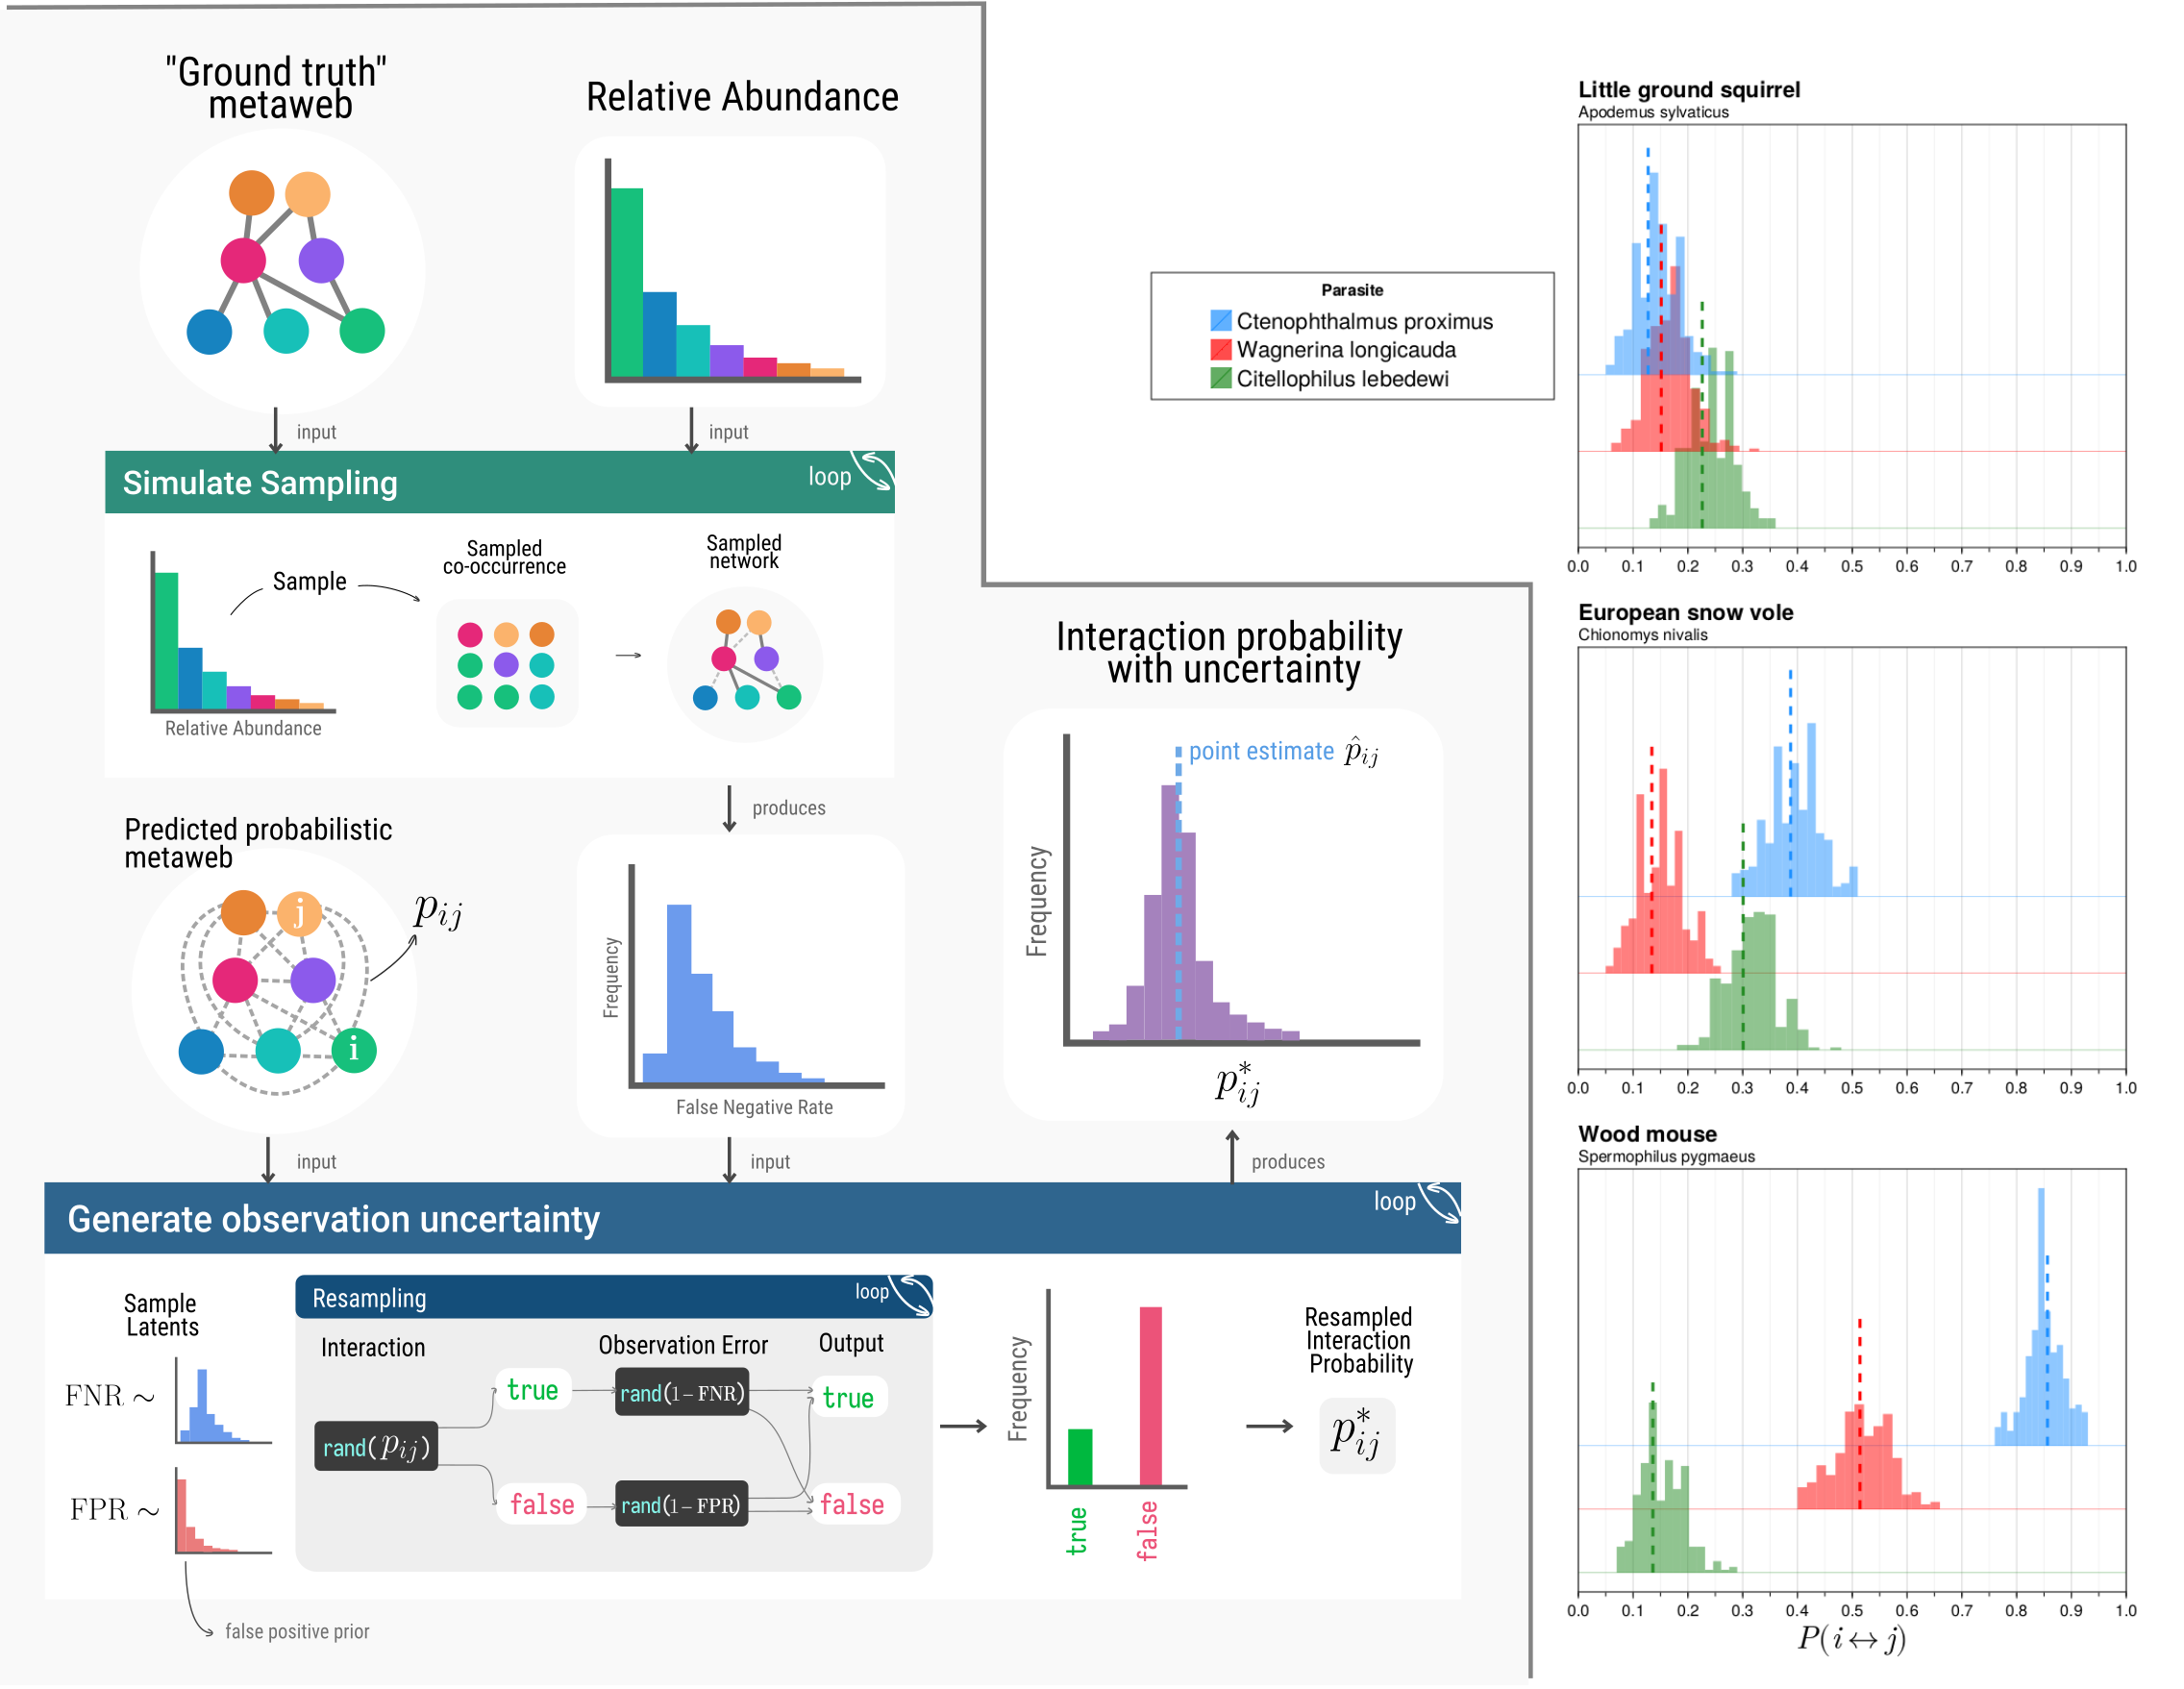
\includegraphics{./figures/uncertainty_sampler.png}
\caption{(A) The process for estimating the false-negative-rate (FNR)
for an interaction dataset consisting of \(N\) total observed
interactions. (B) The method for resampling interaction probability
based on estimates of false-negative and false-positive rates. (C) The
method for interaction probability resampling applied to three mammals
and three parasites from the Hadfield \emph{et al.} (2014)
dataset.}\label{fig:resampling_concept}
}
\end{figure}

We then consider the output prediction from an arbitrary prediction
model, which is the probability \(p_{ij}\) that two species \(i\) and
\(j\) interact. To get an estimate of \(p_{ij}\) that accounts for
observation error, we resample the probability of each interaction
\(p_{ij}\) by simulating a set of several `particles,' where each
particle is a realization of an interaction occurring (either true or
false with probabilities \(p_{ij}\) and \(1-p_{ij}\) respectively) and
then being correctly observed with probabilities given by \(p_{fp}\) and
\(p_{fn}\) to yield a single boolean outcome for each particle.
(``Resampling'' within fig.~\ref{fig:resampling_concept} (B)). Over many
samples of particles, the resulting frequency of `true' outcomes is a
single resample of the interaction probability \(p_{ij}^*\). Across
several samples each of several particles, this forms a distribution of
probabilities which are adjusted by the true and false negative rates.

There is also an analytic way to approximate this distribution using the
normal approximation to binomial. As a reminder, as the total number of
samples \(N\) from a binomial distribution for \(n\) trials with success
probability \(p\) from approaches infinity, the sum of total successes
across all samples approaches a normal distribution with mean \(np\) and
variance \(np(1-p)\). We can use this to correct the estimate \(p_{ij}\)
based on the expected false-negative-rate \(p_{fn}\) and false-positive
rate \(p_{fp}\) to obtain the limiting distribution as the number of
resamples approaches infinity for the resampled \(p_{ij}^*\) for a given
number of particles \(n_p\). We do this by first adjusting for the rates
of observation error to get the mean resampled probability,
\(\mathbb{E}[{p_{ij}^*}]\), as

\[
\mathbb{E}[{p_{ij}^*}] = p_{ij}(1-p_{fp})+ (1-p_{ij})p_{fn}
\]

which yields the normal approximation

\[
\sum_{i=1}^{n_p} p_{ij}^* \sim \mathcal{N}\bigg(n_p \cdot \mathbb{E}[p_{ij}^*], \sqrt{n_p\mathbb{E}[p_{ij}^*] (1- \mathbb{E}[p_{ij}^*])}\bigg)
\]

which then can be converted back to a distribution of frequency of
successes to yield the final approximation

\begin{equation}\protect\hypertarget{eq:eq1}{}{p_{ij}^* \sim \mathcal{N}\bigg( \mathbb{E}[p_{ij}^*] , \sqrt{\frac{\mathbb{E}[p_{ij}^*]
(1-\mathbb{E}[p_{ij}^*] )}{n_p}} \bigg)}\label{eq:eq1}\end{equation}

We can then further truncate to remain on the interval \((0,1)\) (as the
output is a probability, although in practice often the probability mass
outside \((0,1)\) is exteremly low. As an example case study, we use a
boosted-regression-tree to predict interactions in a host-parasite
network (Hadfield \emph{et al.} 2014) (with features derived in the same
manner as Strydom \emph{et al.} (2021) derives features on this data) to
produce a set of interaction predictions. We then applied this method to
a set of a few resampled interaction probabilities between mammals and
parasite species shown in figure fig.~\ref{fig:resampling_concept}(C).

Why is this useful? For one, this analytic method avoids the extra
computation required by simulating samples from this distribution
directly. Further, it enables continuous exanination of the number of
particles \(n_p\) as a uncertainty width. The natural analogue for the
number of particles sampled is the number of observations of
co-occurrence for a given pair of species---the fewer the particles, the
higher the variance of the resulting approximation. The normal
approximation is undefined for 0 particles (i.e.~0 observations
co-occurrence), although as \(n_p\) approaches \(0\) the approxated
normal (once truncated) approaches a uniform distribution on the
interval \((0,1)\), the maximum entropy distribution where we have no
information about the possibility of an interaction.

This also has implications for what we mean by `uncertainty' in
interaction predictions. A model's prediction can be `uncertain' in two
different ways: (1) the model's predictions may have high variance, or
(2) the model's predictions may be centered around a probability of
interaction of \(0.5\), where we are the most unsure about whether this
interaction exists. Improving the incorporation of different forms of
uncertainty in probabilistic interaction predictions seems a necessary
next step toward understanding what pairs of species we know the least
about, in order to prioritize sampling to provide the most new
information possible.

\hypertarget{positive-associations-in-co-occurrence-increase-the-false-negative-rate}{%
\section{Positive associations in co-occurrence increase the
false-negative-rate}\label{positive-associations-in-co-occurrence-increase-the-false-negative-rate}}

The model above doesn't consider the possibility that there are positive
or negative associations which shift the probability of species
cooccurrence away from what is expected based on their relative
abundances due to their interaction (Cazelles \emph{et al.} 2016).
However, here we demonstrate that the probability of having a
false-negative can be higher if there is some positive association in
the occurrence of species \(A\) and \(B\). If we denote the probability
that we observe the co-occurrence of two species \(A\) and \(B\) as
\(P(AB)\) and if there is no association between the marginal
probabilities of observing \(A\) and observing \(B\), denoted \(P(A)\)
and \(P(B)\) respectively, then the probability of observing their
co-occurrence is the product of the marginal probabilities for each
species, \(P(AB) = P(A)P(B)\). In the other case where there is some
positive strength of association between observing both \(A\) and \(B\)
because this interaction is ``important'' for each species, then the
probability of observation both \(A\) and \(B\), \(P(AB)\), is greater
than \(P(A)P(B)\) as \(P(A)\) and \(P(B)\) are not independent and
instead are positively correlated, i.e.~\(P(AB)> P(A)P(B)\). In this
case, the probability of observing a single false-negative in our naive
model from fig.~\ref{fig:geometric}(A) is \(p_{fn}= 1-P(AB)\), which due
to the above inequality implies \(p_{fn}>1-P(A)P(B)\). This indicates an
increasingly greater probability of a false negative as the strength of
association gets stronger, \(P(AB) \to P(AB) \gg P(A)P(B)\). However,
this still does not consider variation in species abundance in space and
time (Poisot \emph{et al.} 2015). If positive or negative associations
between species structure variation in the distribution of \(P(AB)\)
across space/time, then the spatial/temporal biases induced by data
collection would further impact the realized false-negative-rate, as the
probability of false negative would not be constant for each pair of
species across sites.

To test for these positive associations in data we scoured Mangal for
datasets with many spatial or temporal replicates of the same system,
which led the the resulting seven datasets set in figure
fig.~\ref{fig:mangal}. For each dataset, we compute the marginal
probability \(P(A)\) of occurrence of each species \(A\) across all
networks in the dataset. For each pair of interacting species \(A\) and
\(B\), we then compute and compare the probability of co-occurrence if
each species occurs independently, \(P(A)P(B)\), to the empirical joint
probability of co-occurrence, \(P(AB)\). Following our analysis above,
if \(P(AB)\) is greater than \(P(A)P(B)\), then we expect our neutral
estimates of the FNR above to underestimate the realized FNR. In
fig.~\ref{fig:mangal}, we see the difference between \(P(AB)\) and
\(P(A)P(B)\) for the seven suitable datasets with enough spatio-temporal
replicates and a shared taxonomic backbone (meaning all individual
networks use common species identifiers) found on Mangal to perform this
analysis. Further details about each dataset are reported in
tbl.~\ref{tbl:id}.

In each of these datasets, the joint probability of co-occurrence
\(P(AB)\) is decisively greater than our expectation if species co-occur
in proportion to their relative abundance \(P(A)P(B)\). This suggests
that there may not be as many ``neutrally forbidden links'' (Canard
\emph{et al.} 2012) as we might think, and that the reason we do not
have records of interactions between rare species is probably due to
observation error. This has serious ramifications for the widely
observed property of nestedness seen in bipartite networks (Bascompte \&
Jordano 2007)---perhaps the reason we have lots of observations between
generalists is because they are more abundant, and this is particularly
relevant as we have strong evidence that generalism drives abundance
(Song \emph{et al.} 2022a), not vice-versa.

\begin{figure}
\hypertarget{fig:mangal}{%
\centering
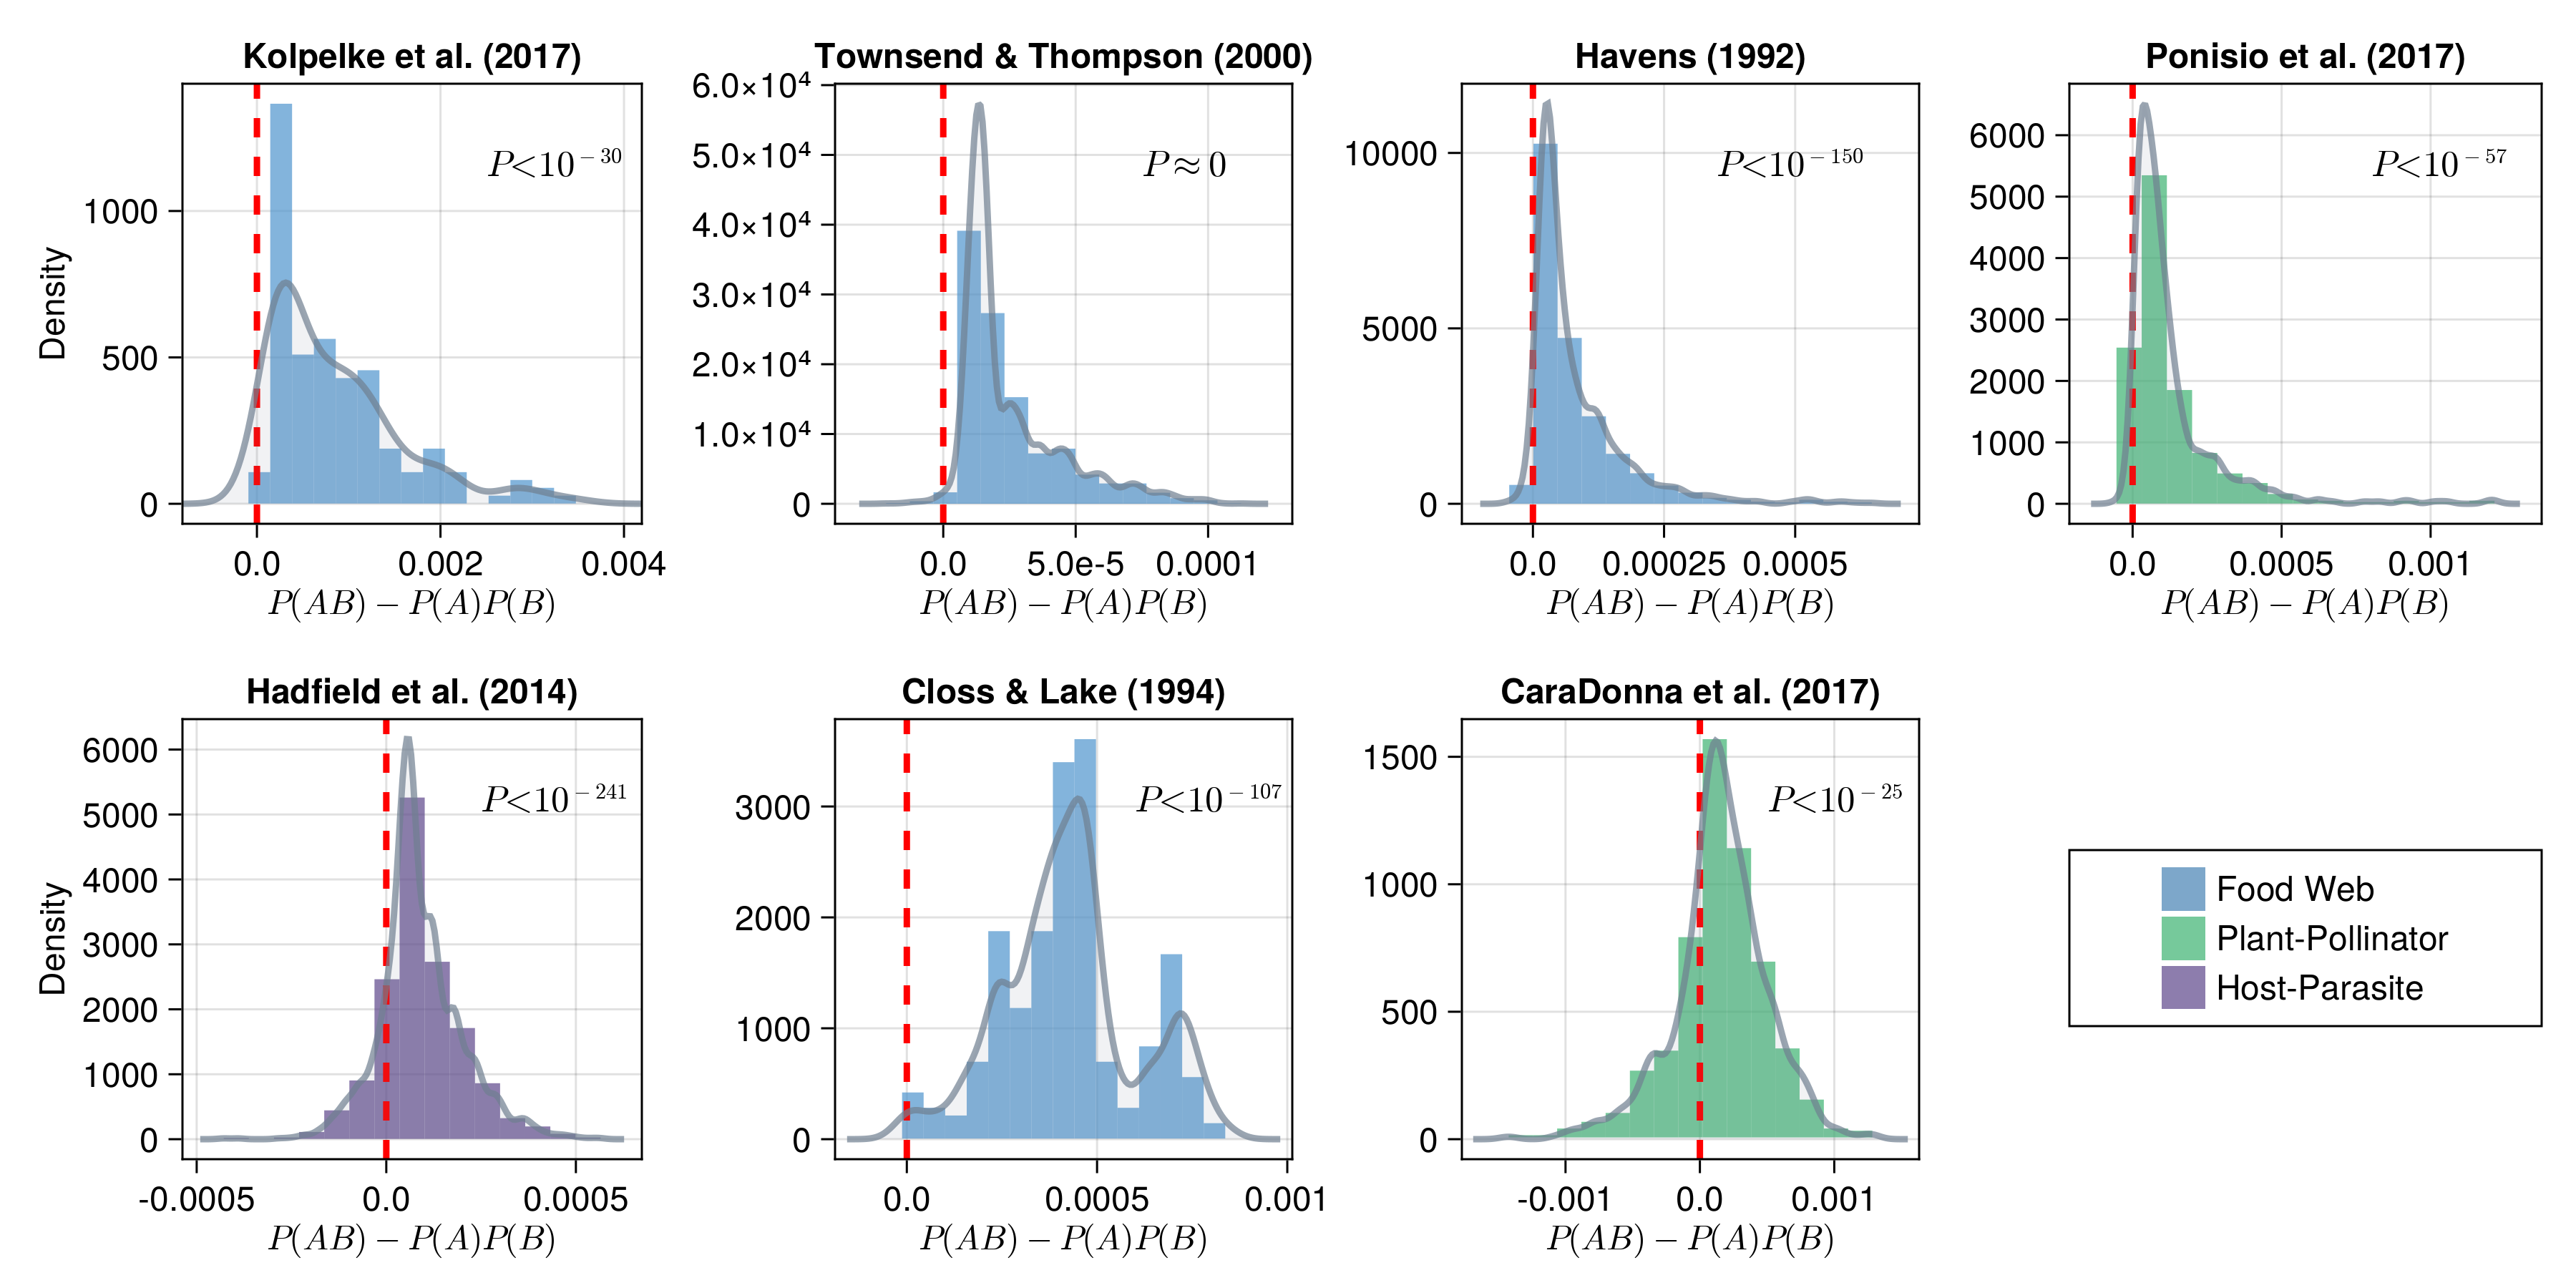
\includegraphics{./figures/fig2.png}
\caption{The difference between joint-probability of co-occurrence
(\(P(AB)\)) and expected probability of co-occurrence under independence
(\(P(A)P(B)\)) for interacting species for each dataset. The red-dashed
line indicates 0 (no association). Each histogram represents a density,
meaning the area of the entire curve sums to 1. The continuous density
estimate (computed using local smoothing) is shown in grey. The p-value
on each plot is the result of a one-sided t-test comparing the mean of
each distribution to 0.}\label{fig:mangal}
}
\end{figure}

\hypertarget{tbl:id}{}
\begin{longtable}[]{@{}ccccccccc@{}}
\caption{\label{tbl:id}The datasets used in the above analysis (Fig 2).
The table reports the type of each dataset, the total number of networks
in each dataset \((N)\), the total species richness in each dataset
\((S)\), the connectance of each metaweb (all interactions across the
entire spatial-temporal extent) \((C)\), the mean species richness
across each local network \(\bar{S}\), the mean connectance of each
local network \(\bar{C}\), the mean \(\beta\)-diversity among
overlapping species across all pairs of network species
(\(\bar{\beta}_{OS}\)), and the mean \(\beta\)-diversity among all
species in the metaweb (\(\bar{\beta}_{WN}\)). Both metrics are computed
using KGL \(\beta\)-diversity (Koleff \emph{et al.}
2003)}\tabularnewline
\toprule
Network & Type & \(N\) & \(S\) & \(C\) & \(\bar{S}\) & \(\bar{C}\) &
\(\bar{\beta}_{OS}\) & \(\bar{\beta}_{WN}\)\tabularnewline
\midrule
\endfirsthead
\toprule
Network & Type & \(N\) & \(S\) & \(C\) & \(\bar{S}\) & \(\bar{C}\) &
\(\bar{\beta}_{OS}\) & \(\bar{\beta}_{WN}\)\tabularnewline
\midrule
\endhead
Kopelke \emph{et al.} (2017) & Food Web & 100 & 98 & 0.037 & 7.87 &
0.142 & 1.383 & 1.972\tabularnewline
Thompson \& Townsend (2000) & Food Web & 18 & 566 & 0.014 & 80.67 &
0.049 & 1.617 & 1.594\tabularnewline
Havens (1992) & Food Web & 50 & 188 & 0.065 & 33.58 & 0.099 & 1.468 &
1.881\tabularnewline
Ponisio \emph{et al.} (2017) & Pollinator & 100 & 226 & 0.079 & 23.0 &
0.056 & 1.436 & 1.870\tabularnewline
Hadfield \emph{et al.} (2014) & Host-Parasite & 51 & 327 & 0.085 & 32.71
& 0.337 & 1.477 & 1.952\tabularnewline
Closs \& Lake (1994) & Food Web & 12 & 61 & 0.14 & 29.09 & 0.080 & 1.736
& 1.864\tabularnewline
CaraDonna \emph{et al.} (2017) & Pollinator & 86 & 122 & 0.18 & 21.42 &
0.312 & 1.527 & 1.907\tabularnewline
\bottomrule
\end{longtable}

\hypertarget{the-impact-of-false-negatives-on-network-properties-and-prediction}{%
\section{The impact of false-negatives on network properties and
prediction}\label{the-impact-of-false-negatives-on-network-properties-and-prediction}}

Here, we assess the effect of false-negatives on our ability to make
predictions about interactions, as well as their effect on network
structure. The prevalence of false-negatives in data is the catalyst for
interaction prediction in the first place, and as a result methods have
been proposed to counteract this bias (Stock \emph{et al.} 2017; Poisot
\emph{et al.} 2022). However, it is feasible that the FNR in a given
dataset is so high that it could induce too much noise for an
interaction prediction model to detect the signal of possible
interaction between species.

To test this we use the dataset from Hadfield \emph{et al.} (2014) that
describes host-parasite interaction networks sampled across 51 sites,
and the same method as Strydom \emph{et al.} (2021) to extract latent
features for each species in this dataset based on applying PCA to the
co-occurrence matrix. We then predict a metaweb (equivalent to
predicting true or false for an interaction between each species pair,
effectively a binary classification problem) from these species-level
features using four candidate models for binary classification---three
often used machine-learning (ML) methods (Boosted Regression Tree (BRT),
Random Forest (RF), Decision Tree (DT)), and one naive model from
classic statistics (Logistic Regression (LR)). Each of the ML models are
bootstrap aggregated (or bagged) with 100 replicates each. We partition
the data into 80-20 training-test split, and then seed the training data
with false negatives at varying rates, but crucially do nothing to the
test data. We fit all of these models using MLJ.jl, a high-level Julia
framework for a wide-variety of ML models (Blaom \emph{et al.} 2020). We
evaluate the efficacy of these models using two common measures of
binary classifier performance: the area under the receiver-operator
curve (ROC-AUC) and the area under the precision-recall curve (PR-AUC),
for more details see Poisot (2022). Here, PR-AUC is slightly more
relevant as it is a better indicator of prediction of false-negatives.
The results of these simulations are shown in
fig.~\ref{fig:addedfnr}(A\&B).

\begin{figure}
\hypertarget{fig:addedfnr}{%
\centering
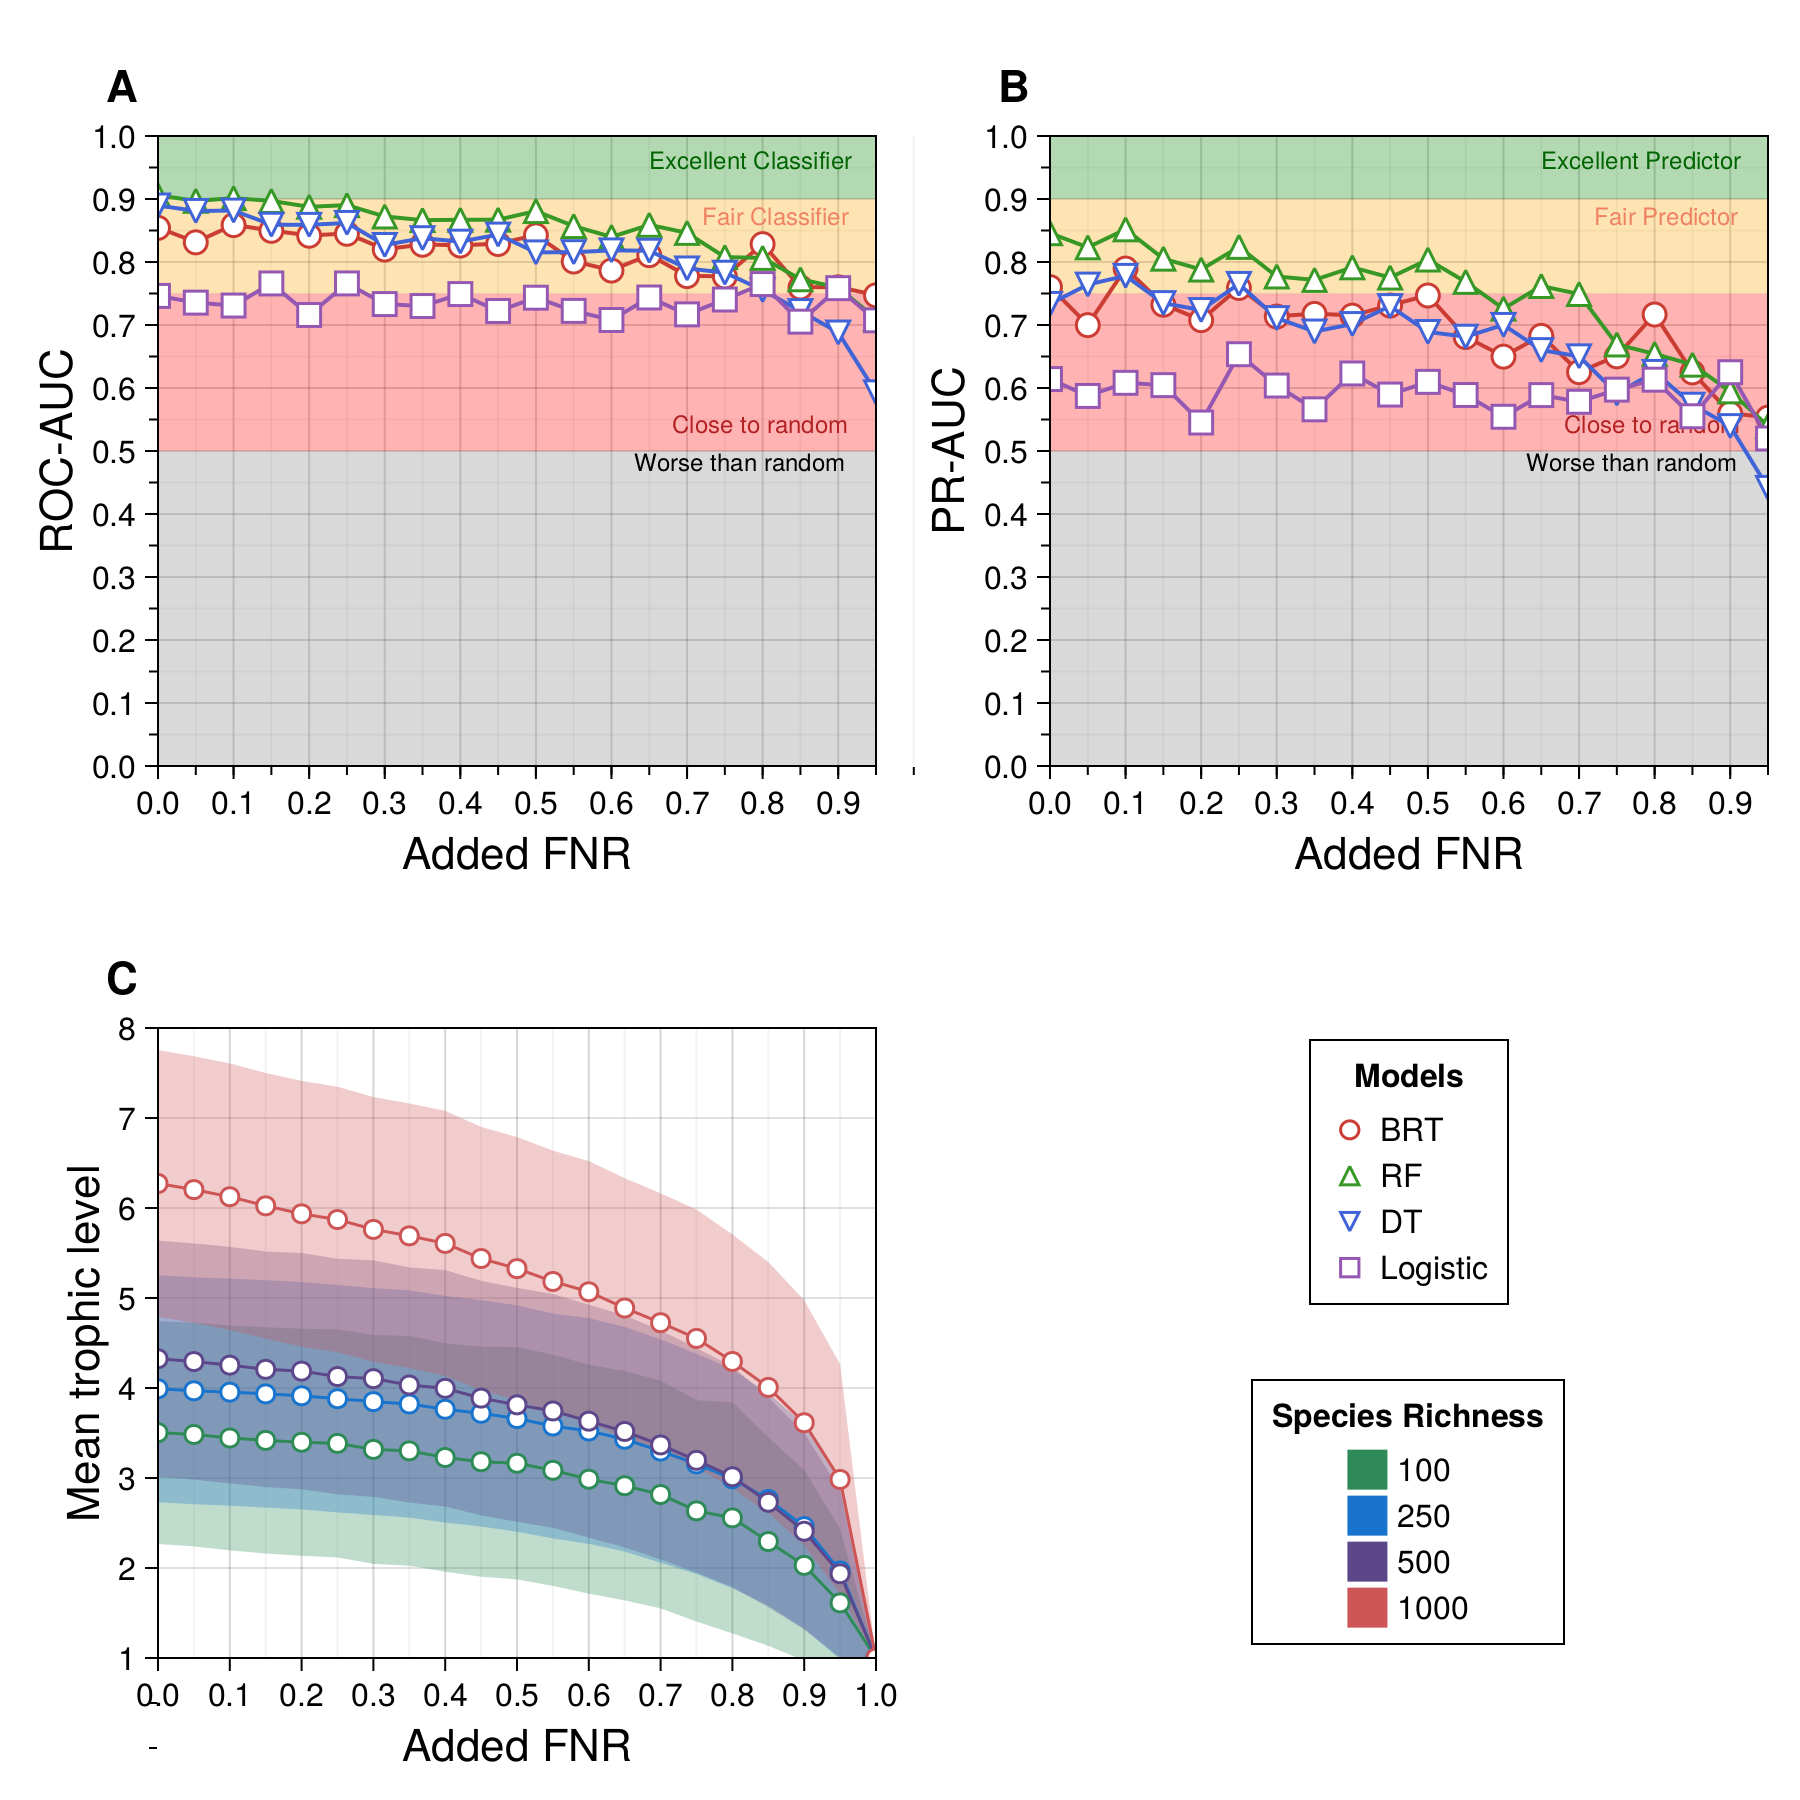
\includegraphics{./figures/fig3.png}
\caption{\textbf{(A)} The area-under the receiver-operator curve
(ROC-AUC) and \textbf{(B)} The area-under the precision-recall curve
(PR-AUC; right) for each different predictive model (colors/shapes)
across a spectrum of the proportion of added false-negatives (x-axis).
\textbf{(C)} The mean trophic-level of all species in a network
generated with the niche model across different species richnesses
(colors). For each value of the FNR, the mean trophic level was computed
across 50 replicates. The shaded region for each line is one
standard-deviation across those replicates.}\label{fig:addedfnr}
}
\end{figure}

One interesting result seen in fig.~\ref{fig:addedfnr}(A\&B) is that the
ROC-AUC value does not approach random in the same way the PR-AUC curve
does as we increase the added FNR. The reason for this is that ROC-AUC
is fundamentally not as useful a metric in assessing predictive capacity
as PR-AUC. As we keep adding more false-negatives, the network
eventually becomes a zeros matrix, and these models can still learn to
predict ``no-interaction'' for all possible species pairs, which does
far better than random guessing (ROC-AUC = 0.5) in terms of the false
positive rate (one of the components of ROC-AUC). This highlights a more
broad issue of label class imbalance, meaning there are far more
non-interactions than interactions in data. A full treatment of the
importance of class-balance is outside the scope of this paper, but is
explored in-depth in Poisot (2022).

Although these ML models are surprisingly performant at link prediction
given their simplicity, there have been several major developments in
applying deep-learning methods to many tasks in network inference and
prediction---namely graph-representation learning (GRL, Khoshraftar \&
An (2022)) and graph convolutional networks (Zhang \emph{et al.} 2019).
At this time, these advances can not yet be applied to ecological
networks because they require far more data than we currently have. We
already have lots of features that could be used as inputs into these
models (i.e.~species level data about occurrence, genomes, abundance,
etc.), but our network datasets barely get into the hundreds of local
networks sampled across space and time (tbl.~\ref{tbl:id}). Once we
start to get into the thousands, these models will become more useful,
but this can only be done with systematic monitoring of interactions.
This again highlights the need to optimize our sampling effort to
maximize the amount of information contained in our data given the
expense of sampling interactions.

We also consider how the FNR affects network properties. In
fig.~\ref{fig:addedfnr}(C) we see the mean trophic level across networks
simulated using the niche model (as above), across a spectrum of FNR
values. In addition to the clear dependence on richness, we see that
mean trophic level, despite varying widely between niche model
simulations, tends to be relatively robust to false-negatives and does
not deviate widely from the true value until very large FNRs,
i.e.~\(p_{fn} > 0.7\). This is not entirely unsurprising. Removing links
randomly from a food-web is effectively the inverse problem of the
emergence of a giant component (more than half of the nodes are in a
connected network) in random graphs (see Li \emph{et al.} (2021) for a
thorough review). The primary difference being that we are removing
edges, not adding them, and thus we are witnessing the dissolution of a
giant component, rather than the emergence of one. Further applications
of percolation theory (Li \emph{et al.} 2021) to the topology of sampled
ecological networks could improve our understanding of how
false-negatives impact the inferences about the structure and dynamics
on these networks.

\hypertarget{discussion}{%
\section{Discussion}\label{discussion}}

Species interactions enable the persistence and functioning of
ecosystems, but our understanding of interactions is limited due to the
intrinsic difficulty of sampling them. Here we have provided a null
model for the expected number of false-negatives in an interaction
dataset. We demonstrated that we expect many false-negatives in species
interaction datasets purely due to the intrinsic variation of abundances
within a community. We also, for the first time to our knowledge,
measured the strength of association between co-occurrence and
interactions (Cazelles \emph{et al.} 2016) across many empirical
systems, and found that these positive associations are both very
common, and showed algebraically that they increase the realized FNR. We
have also shown that false-negatives could further impact our ability to
both predict interactions and infer properties of the networks, which
highlights the need for further research into methods for correcting
this bias in existing data.

A better understanding of how false-negatives impact species interaction
data is a practical necessity---both for inference of network structure
and dynamics, but also for prediction of interactions by using species
level information. False-negatives could pose a problem for many forms
of inference in network ecology. For example, inferring the dynamic
stability of a network could be prone to error if the observed network
is not sampled ``enough.'' What exactly ``enough'' means is then
specific to the application, and should be assessed via methods like
those here when designing samples. Further, predictions about network
rewiring (Thompson \& Gonzalez 2017) due to range shifts in response to
climate change could be error-prone without accounting for interactions
that have not been observed but that still may become climatically
infeasible. As is evident from fig.~\ref{fig:geometric}(A), we can never
guarantee there are no false-negatives in data. In recent years, there
has been interest toward explicitly accounting for false-negatives in
models (Stock \emph{et al.} 2017; Young \emph{et al.} 2021), and a
predictive approach to networks---rather than expecting our samples to
fully capture all interactions (Strydom \emph{et al.} 2021). As a
result, better models for predicting interactions are needed for
interaction networks. This includes explicitly accounting for
observation error (Johnson \& Larremore 2021)---certain classes of
models have been used to reflect hidden states which account for
detection error in occupancy modeling (Joseph 2020), and could be
integrated in the predictive models of interactions in the future.

This work has several practical consequences for the design of surveys
for species' interactions. Simulating the process of observation could
be a powerful tool for estimating the sampling effort required by a
study that takes relative abundance into account, and provides a null
baseline for expected FNR. It is necessary to take the size of the
species pool into account when deciding how many total samples is
sufficient for an ``acceptable'' FNR (fig.~\ref{fig:geometric}(C \& D)).
Further the spatial and temporal turnover of interactions means any
approach to sampling prioritization must be spatiotemporal. We
demonstrated earlier that observed negatives outside of the range of
both species aren't informative, and therefore using species
distribution models could aid in this spatial prioritization of sampling
sites.

We also should address the impact of false-negatives on the inference of
process and causality in community ecology. We demonstrated that in
model food webs, false-negatives do not impact the measure of total
trophic levels until very high FNR (figure fig.~\ref{fig:addedfnr}(C)),
although we cannot generalize this further to other properties. This has
immediate practical concern for how we design what taxa to sample---does
it matter if the sampled network is fully connected? It has been shown
that the stability of subnetworks can be used to infer the stability of
the metaweb paper beyond a threshold of samples (Song \emph{et al.}
2022b). But does this extend to other network properties? And how can we
be sure we are at the threshold at which we can be confident our sample
characterizes the whole system? We suggest that modeling observation
error as we have done here can address these questions and aid in the
design of samples of species interactions. To try to survey to avoid all
false-negatives is a fool's errand. Species ranges overlap to form
mosaics, which themselves are often changing in time. Communities and
networks don't end in space, and the interactions that connect species
on the `periphery' of a given network to species outside the spatial
extent of a given sample will inevitably appear as false-negatives in
practical samples. The goal should instead be to sample a system enough
to have a statistically robust estimate of the current state and
empirical change over time of an ecological community at a given spatial
extent and temporal resolution, and to determine what the sampling
effort required should be prior to sampling.

Our work highlights the need for a quantitatively robust approach to
sampling design, both for interactions (Jordano 2016) and all other
aspects of biodiversity (Carlson \emph{et al.} 2020). As anthropogenic
forces create rapid shifts in our planet's climate and biosphere, this
is an imperative to maximize the amount of ecological information we get
in our finite samples, and make our inferences and decisions based on
this data as robust as possible. Where we choose to sample, and how
often we choose to sample there, has strong impacts on the inferences we
make from data. Incorporating a better understanding of sampling effort
and bias to the design of biodiversity monitoring systems, and the
inference and predictive models we apply to this data, is imperative in
understanding how biodiversity is changing, and making forecasts that
can guide conservation action.

\hypertarget{acknowledgements}{%
\section{Acknowledgements}\label{acknowledgements}}

AG \& MDC acknowledge the support of the Liber Ero Chair for
Biodiversity conservation and NSERC.

\hypertarget{references}{%
\section*{References}\label{references}}
\addcontentsline{toc}{section}{References}

\hypertarget{refs}{}
\begin{CSLReferences}{1}{0}
\leavevmode\hypertarget{ref-Banville2021ManJl}{}%
Banville, F., Vissault, S. \& Poisot, T. (2021). Mangal.jl and
EcologicalNetworks.jl: Two complementary packages for analyzing
ecological networks in Julia. \emph{Journal of Open Source Software}, 6,
2721.

\leavevmode\hypertarget{ref-Bascompte2007PlaMut}{}%
Bascompte, J. \& Jordano, P. (2007). Plant-Animal Mutualistic Networks:
The Architecture of Biodiversity. \emph{Annual Review of Ecology,
Evolution, and Systematics}, 38, 567--593.

\leavevmode\hypertarget{ref-Becker2021OptPre}{}%
Becker, D.J., Albery, G.F., Sjodin, A.R., Poisot, T., Bergner, L.M.,
Dallas, T.A., \emph{et al.} (2021). Optimizing predictive models to
prioritize viral discovery in zoonotic reservoirs.

\leavevmode\hypertarget{ref-Bezanson2015JulFre}{}%
Bezanson, J., Edelman, A., Karpinski, S. \& Shah, V.B. (2015). Julia: A
Fresh Approach to Numerical Computing.

\leavevmode\hypertarget{ref-Blanchet2020CooNot}{}%
Blanchet, F.G., Cazelles, K. \& Gravel, D. (2020). Co-occurrence is not
evidence of ecological interactions. \emph{Ecology Letters}, 23,
1050--1063.

\leavevmode\hypertarget{ref-Blaom2020MljJul}{}%
Blaom, A.D., Kiraly, F., Lienart, T., Simillides, Y., Arenas, D. \&
Vollmer, S.J. (2020). MLJ: A Julia package for composable machine
learning. \emph{Journal of Open Source Software}, 5, 2704.

\leavevmode\hypertarget{ref-Boakes2015InfSpe}{}%
Boakes, E.H., Rout, T.M. \& Collen, B. (2015). Inferring species
extinction: The use of sighting records. \emph{Methods in Ecology and
Evolution}, 6, 678--687.

\leavevmode\hypertarget{ref-Canard2012EmeStr}{}%
Canard, E., Mouquet, N., Marescot, L., Gaston, K.J., Gravel, D. \&
Mouillot, D. (2012). Emergence of Structural Patterns in Neutral Trophic
Networks. \emph{PLOS ONE}, 7, e38295.

\leavevmode\hypertarget{ref-CaraDonna2017IntRew}{}%
CaraDonna, P.J., Petry, W.K., Brennan, R.M., Cunningham, J.L.,
Bronstein, J.L., Waser, N.M., \emph{et al.} (2017). Interaction rewiring
and the rapid turnover of plantpollinator networks. \emph{Ecology
Letters}, 20, 385--394.

\leavevmode\hypertarget{ref-Carlson2020WhaWou}{}%
Carlson, C.J., Dallas, T.A., Alexander, L.W., Phelan, A.L. \& Phillips,
A.J. (2020). What would it take to describe the global diversity of
parasites? \emph{Proceedings of the Royal Society B: Biological
Sciences}, 287, 20201841.

\leavevmode\hypertarget{ref-Cazelles2016TheSpe}{}%
Cazelles, K., Araújo, M.B., Mouquet, N. \& Gravel, D. (2016). A theory
for species co-occurrence in interaction networks. \emph{Theoretical
Ecology}, 9, 39--48.

\leavevmode\hypertarget{ref-Closs1994SpaTem}{}%
Closs, G.P. \& Lake, P.S. (1994). Spatial and Temporal Variation in the
Structure of an Intermittent-Stream Food Web. \emph{Ecological
Monographs}, 64, 1--21.

\leavevmode\hypertarget{ref-deAguiar2019RevBia}{}%
de Aguiar, M.A.M., Newman, E.A., Pires, M.M., Yeakel, J.D., Boettiger,
C., Burkle, L.A., \emph{et al.} (2019). Revealing biases in the sampling
of ecological interaction networks. \emph{PeerJ}, 7, e7566.

\leavevmode\hypertarget{ref-Gauzens2013FooAgg}{}%
Gauzens, B., Legendre, S., Lazzaro, X. \& Lacroix, G. (2013). Food-web
aggregation, methodological and functional issues. \emph{Oikos}, 122,
1606--1615.

\leavevmode\hypertarget{ref-Giacomuzzo2021FooWeb}{}%
Giacomuzzo, E. \& Jordán, F. (2021). Food web aggregation: Effects on
key positions. \emph{Oikos}, 130, 2170--2181.

\leavevmode\hypertarget{ref-Griffiths1998SamEff}{}%
Griffiths, D. (1998). Sampling effort, regression method, and the shape
and slope of sizeabundance relations. \emph{Journal of Animal Ecology},
67, 795--804.

\leavevmode\hypertarget{ref-Hadfield2014TalTwo}{}%
Hadfield, J.D., Krasnov, B.R., Poulin, R. \& Nakagawa, S. (2014). A Tale
of Two Phylogenies: Comparative Analyses of Ecological Interactions.
\emph{The American Naturalist}, 183, 174--187.

\leavevmode\hypertarget{ref-Havens1992ScaStr}{}%
Havens, K. (1992). Scale and Structure in Natural Food Webs.
\emph{Science}, 257, 1107--1109.

\leavevmode\hypertarget{ref-Johnson2021BayEst}{}%
Johnson, E.K. \& Larremore, D.B. (2021). Bayesian estimation of
population size and overlap from random subsamples.

\leavevmode\hypertarget{ref-Jordano2016SamNet}{}%
Jordano, P. (2016). Sampling networks of ecological interactions.
\emph{Functional Ecology}, 30, 1883--1893.

\leavevmode\hypertarget{ref-Joseph2020NeuHie}{}%
Joseph, M.B. (2020). Neural hierarchical models of ecological
populations. \emph{Ecology Letters}, 23, 734--747.

\leavevmode\hypertarget{ref-Kenall2014OpeFut}{}%
Kenall, A., Harold, S. \& Foote, C. (2014). An open future for
ecological and evolutionary data? \emph{BMC Evolutionary Biology}, 14,
66.

\leavevmode\hypertarget{ref-Khoshraftar2022SurGra}{}%
Khoshraftar, S. \& An, A. (2022). A Survey on Graph Representation
Learning Methods.

\leavevmode\hypertarget{ref-Koleff2003MeaBet}{}%
Koleff, P., Gaston, K.J. \& Lennon, J.J. (2003). Measuring beta
diversity for presenceabsence data. \emph{Journal of Animal Ecology},
72, 367--382.

\leavevmode\hypertarget{ref-Kopelke2017FooStr}{}%
Kopelke, J.-P., Nyman, T., Cazelles, K., Gravel, D., Vissault, S. \&
Roslin, T. (2017). Food-web structure of willow-galling sawflies and
their natural enemies across Europe. \emph{Ecology}, 98, 1730--1730.

\leavevmode\hypertarget{ref-Li2021PerCom}{}%
Li, M., Liu, R.-R., Lü, L., Hu, M.-B., Xu, S. \& Zhang, Y.-C. (2021).
Percolation on complex networks: Theory and application. \emph{Physics
Reports}, Percolation on complex networks: Theory and application, 907,
1--68.

\leavevmode\hypertarget{ref-MacDonald2020RevLin}{}%
MacDonald, A.A.M., Banville, F. \& Poisot, T. (2020). Revisiting the
Links-Species Scaling Relationship in Food Webs. \emph{Patterns}, 1.

\leavevmode\hypertarget{ref-Makiola2020KeyQue}{}%
Makiola, A., Compson, Z.G., Baird, D.J., Barnes, M.A., Boerlijst, S.P.,
Bouchez, A., \emph{et al.} (2020). Key Questions for Next-Generation
Biomonitoring. \emph{Frontiers in Environmental Science}, 7.

\leavevmode\hypertarget{ref-Martinez1999EffSam}{}%
Martinez, N.D., Hawkins, B.A., Dawah, H.A. \& Feifarek, B.P. (1999).
Effects of Sampling Effort on Characterization of Food-Web Structure.
\emph{Ecology}, 80, 1044--1055.

\leavevmode\hypertarget{ref-McLeod2021SamAsy}{}%
McLeod, A., Leroux, S.J., Gravel, D., Chu, C., Cirtwill, A.R., Fortin,
M.-J., \emph{et al.} (2021). Sampling and asymptotic network properties
of spatial multi-trophic networks. \emph{Oikos}, 130, 2250--2259.

\leavevmode\hypertarget{ref-Moore2016OptEco}{}%
Moore, A.L. \& McCarthy, M.A. (2016). Optimizing ecological survey
effort over space and time. \emph{Methods in Ecology and Evolution}, 7,
891--899.

\leavevmode\hypertarget{ref-Niedballa2019AssAna}{}%
Niedballa, J., Wilting, A., Sollmann, R., Hofer, H. \& Courtiol, A.
(2019). Assessing analytical methods for detecting spatiotemporal
interactions between species from camera trapping data. \emph{Remote
Sensing in Ecology and Conservation}, 5, 272--285.

\leavevmode\hypertarget{ref-Paine1988RoaMap}{}%
Paine, R.T. (1988). Road Maps of Interactions or Grist for Theoretical
Development? \emph{Ecology}, 69, 1648--1654.

\leavevmode\hypertarget{ref-Poisot2022GuiPre}{}%
Poisot, T. (2022). Guidelines for the prediction of species interactions
through binary classification.

\leavevmode\hypertarget{ref-Poisot2021GloKno}{}%
Poisot, T., Bergeron, G., Cazelles, K., Dallas, T., Gravel, D.,
MacDonald, A., \emph{et al.} (2021). Global knowledge gaps in species
interaction networks data. \emph{Journal of Biogeography}, 48,
1552--1563.

\leavevmode\hypertarget{ref-Poisot2022NetEmb}{}%
Poisot, T., Ouellet, M.-A., Mollentze, N., Farrell, M.J., Becker, D.J.,
Brierly, L., \emph{et al.} (2022). Network embedding unveils the hidden
interactions in the mammalian virome.

\leavevmode\hypertarget{ref-Poisot2015SpeWhy}{}%
Poisot, T., Stouffer, D.B. \& Gravel, D. (2015). Beyond species: Why
ecological interaction networks vary through space and time.
\emph{Oikos}, 124, 243--251.

\leavevmode\hypertarget{ref-Ponisio2017OppAtt}{}%
Ponisio, L.C., Gaiarsa, M.P. \& Kremen, C. (2017). Opportunistic
attachment assembles plantpollinator networks. \emph{Ecology Letters},
20, 1261--1272.

\leavevmode\hypertarget{ref-Savage2004EffBod}{}%
Savage, V.M., Gillooly, J.F., Brown, J.H., West, G.B. \& Charnov, E.L.
(2004). Effects of Body Size and Temperature on Population Growth.
\emph{The American Naturalist}, 163, 429--441.

\leavevmode\hypertarget{ref-Song2022GenDri}{}%
Song, C., Simmons, B.I., Fortin, M.-J. \& Gonzalez, A. (2022a).
Generalism drives abundance: A computational causal discovery approach.
\emph{PLOS Computational Biology}, 18, e1010302.

\leavevmode\hypertarget{ref-Song2022RapMon}{}%
Song, C., Simmons, B.I., Fortin, M.-J., Gonzalez, A., Kaiser-Bunbury,
C.N. \& Saavedra, S. (2022b). Rapid monitoring for ecological
persistence.

\leavevmode\hypertarget{ref-Stephenson2020TecAdv}{}%
Stephenson, P. (2020). Technological advances in biodiversity
monitoring: Applicability, opportunities and challenges. \emph{Current
Opinion in Environmental Sustainability}, Open issue 2020 part A:
Technology Innovations and Environmental Sustainability in the
Anthropocene, 45, 36--41.

\leavevmode\hypertarget{ref-Stock2017LinFil}{}%
Stock, M., Poisot, T., Waegeman, W. \& De Baets, B. (2017). Linear
filtering reveals false negatives in species interaction data.
\emph{Scientific Reports}, 7, 45908.

\leavevmode\hypertarget{ref-Strydom2021RoaPre}{}%
Strydom, T., Catchen, M.D., Banville, F., Caron, D., Dansereau, G.,
Desjardins-Proulx, P., \emph{et al.} (2021). A roadmap towards
predicting species interaction networks (across space and time).
\emph{Philosophical Transactions of the Royal Society B: Biological
Sciences}, 376, 20210063.

\leavevmode\hypertarget{ref-Thompson2017DisGov}{}%
Thompson, P.L. \& Gonzalez, A. (2017). Dispersal governs the
reorganization of ecological networks under environmental change.
\emph{Nature Ecology \& Evolution}, 1, 1--8.

\leavevmode\hypertarget{ref-Thompson2000ResSol}{}%
Thompson, R.M. \& Townsend, C.R. (2000). Is resolution the solution?:
The effect of taxonomic resolution on the calculated properties of three
stream food webs. \emph{Freshwater Biology}, 44, 413--422.

\leavevmode\hypertarget{ref-Volkov2003NeuThe}{}%
Volkov, I., Banavar, J.R., Hubbell, S.P. \& Maritan, A. (2003). Neutral
theory and relative species abundance in ecology. \emph{Nature}, 424,
1035--1037.

\leavevmode\hypertarget{ref-Walther1995SamEff}{}%
Walther, B.A., Cotgreave, P., Price, R.D., Gregory, R.D. \& Clayton,
D.H. (1995). Sampling Effort and Parasite Species Richness.
\emph{Parasitology Today}, 11, 306--310.

\leavevmode\hypertarget{ref-Williams2000SimRul}{}%
Williams, R.J. \& Martinez, N.D. (2000). Simple rules yield complex food
webs. \emph{Nature}, 404, 180--183.

\leavevmode\hypertarget{ref-Willott2001SpeAcc}{}%
Willott, S.j. (2001). Species accumulation curves and the measure of
sampling effort. \emph{Journal of Applied Ecology}, 38, 484--486.

\leavevmode\hypertarget{ref-Young2021RecPla}{}%
Young, J.-G., Valdovinos, F.S. \& Newman, M.E.J. (2021). Reconstruction
of plantpollinator networks from observational data. \emph{Nature
Communications}, 12, 3911.

\leavevmode\hypertarget{ref-Zhang2019GraCon}{}%
Zhang, S., Tong, H., Xu, J. \& Maciejewski, R. (2019). Graph
convolutional networks: A comprehensive review. \emph{Computational
Social Networks}, 6, 11.

\end{CSLReferences}

\end{document}
